%
%
%
%
%
\documentclass[journal,twoside,web]{ieeecolor}
\usepackage{generic}

%
\usepackage{amsmath,amssymb,amsfonts}
\usepackage{booktabs}
\usepackage{array}
\usepackage{tabularx}
\usepackage{longtable}
\usepackage{graphicx}
\usepackage{float}
\usepackage{textcomp}
\usepackage{xurl}
\usepackage{xcolor}
\newcommand{\rev}[1]{\textcolor{red}{#1}}
\usepackage[hidelinks]{hyperref}
%
\makeatletter
\let\NAT@parse\undefined
\makeatother
\usepackage[numbers,sort&compress]{natbib}

%
\graphicspath{{../e_result/figures/}{../figures/}{../images/}}
%
%
\makeatletter
\AtBeginDocument{\def\input@path{{../}}}
\makeatother

\markboth{\hskip25pc IEEE TRANSACTIONS AND JOURNALS}
{Balandong \MakeLowercase{\textit{et al.}}: Epoch-Aware Threshold Estimation for Blink Detection}

\makeatletter%
\begin{document}

%
\title{\rev{Epoch-Aware Threshold Estimation for Blink Detection in Simulated-Driving EEG}}

%
\author{Rodney Petrus Balandong, Nur Syahirah Roslan, Syaimaa' Solehah Mohd Radzi,
Muhamad Hafiz Abd Latif,
%
    and Tong Boon Tang
\thanks{This research was supported by the Ministry of Higher Education (MOHE)
under the Fundamental Research Grant Scheme -- Early Career Researcher
(FRGS-EC) with the project code (FRGC026-2024).}
\thanks{Rodney Petrus Balandong is with the Faculty of Science and Natural
Resources, Universiti Malaysia Sabah, 88400 Kota Kinabalu, Sabah, Malaysia (corresponding
author, e-mail: balandong@ums.edu.my).}
\thanks{Nur Syahirah Roslan is with the Department of Information Systems,
Faculty of Information and Communication Technology, Universiti Tunku Abdul
Rahman, Perak, Malaysia.}
%
%
\thanks{Syaimaa' Solehah Mohd Radzi, Muhamad Hafiz Abd Latif, and Tong Boon
Tang are with the Centre for Intelligent Signal and Imaging Research (CISIR),
Universiti Teknologi PETRONAS, 32610 Seri Iskandar, Perak, Malaysia.}}

\maketitle

%
\begin{abstract}
    In fatigue-driving research, blink activity in electroencephalography (EEG) is treated as a marker of driver fatigue rather than as noise. Amplitude thresholding is among the most straightforward and widely used approaches for detecting blinks in EEG.
\rev{However, existing thresholding methods typically estimate a single amplitude threshold from continuous signals in which blink-heavy and blink-free segments are pooled together, which may shift the operating point of the resulting detector.} This study presents an epoch-aware, three-stage pipeline that avoids this dilution by estimating thresholds only from epochs likely to contain blink activity. The pipeline first identifies candidate epochs through multi-channel peak-to-peak amplitude screening, then derives a robust threshold for each channel from these candidate epochs, and finally applies each threshold to its corresponding channel across all epochs to extract channel-wise blink regions.
\rev{The proposed pipeline was compared with two continuous-signal baselines, a BLINKER-derived threshold baseline and the MNE routine, on the full 32-channel montage using two simulated-driving EEG corpora, an internally collected dataset and a public dataset, with performance evaluated through event-level overlap matching and macro-averaged $F_1$. The proposed pipeline achieved macro-$F_1$ scores of 88.25\% on the internal dataset and 80.68\% on the public dataset, significantly outperforming both baselines on both corpora. These results indicate that the complete proposed configuration achieved higher event-level $F_1$ than the examined baselines under the evaluated offline protocol; a matched ablation would be needed to attribute the advantage specifically to epoch screening.}
\end{abstract}
 
\begin{IEEEkeywords}
%
\rev{blink detection, electroencephalography, epoch-aware detection, simulated
driving, threshold selection}
\end{IEEEkeywords}

%
%
%
\section{Introduction}

%
Blinking is a physiological process that involves the closure and reopening of the eyelids \citep{nystrm2024what}. Its primary functions are to protect the ocular surface, maintain corneal moisture, and support visual comfort \citep{nystrm2024what}. Beyond these physiological functions, blink behaviour has been increasingly recognised as an important indicator in fatigue-driving research \citep{alyan2023blink,tian2021fatigue}. Variations in blink-related features, such as blink frequency, blink duration, eye-closure duration, and blink patterns, can reflect changes in alertness and cognitive state \citep{alyan2023blink,ren2019comparison}.
In the context of driving fatigue, increasing fatigue levels are often associated with slower and more prolonged blinks, which may reflect reduced vigilance and an elevated risk of impaired driving performance~\citep{alyan2023blink}.
Therefore, blink behaviour provides a useful and non-invasive marker for monitoring driver fatigue \citep{shahbakhti2023fusion,tian2021fatigue}.
 
%
In the neuroscience study of fatigue driving, blink activity can be captured through external methods, such as camera-based eye monitoring, or through electrophysiological recordings, particularly electroencephalography and electrooculography~\citep{tian2021fatigue,shahbakhti2023fusion}. Although EEG is mainly used to measure brain activity, blink-related components are often present in EEG signals because eyelid movements and eye movements generate strong electrical potentials~\citep{croft2000removal,akuthota2023artifacts}.
%
As a result, blink information can be extracted from EEG recordings, either by analysing the ocular components embedded in the EEG signal ~\citep{agarwal2019blink,shahbakhti2023fusion}.
This makes EEG recordings valuable not only for studying neural activity during fatigue but also for identifying blink-related markers associated with drowsiness~\citep{ko2020eyeblink,alyan2023blink}.
 
%
It is important to distinguish between two major perspectives on blink activity in the existing literature~\citep{croft2000removal,tian2021fatigue}.
In many EEG studies, blink-related activity is treated as an artifact because it contaminates neural signals and may interfere with the interpretation of brain activity~\citep{croft2000removal,akuthota2023artifacts}. In such cases, blink components are commonly removed during EEG preprocessing~\citep{croft2000removal,klein2013reliable}. However, in fatigue-driving studies, blink activity can also be treated as meaningful information rather than noise~\citep{tian2021fatigue,shahbakhti2023fusion}. From this perspective, blink events are identified, extracted, and analysed as potential indicators of driver fatigue~\citep{ko2020eyeblink,shahbakhti2023fusion}. Blink detection methods can generally be classified into machine-learning-based, morphology-based, and thresholding-based approaches~\citep{agarwal2019blink,zhang2023method}. Machine learning methods rely on trained models to classify blink events, while morphology-based methods identify blinks based on their characteristic waveform shape~\citep{rashida2023quantitative,jiang2023eyeblink}. Thresholding-based methods, in contrast, detect
candidate blink events when the signal amplitude exceeds a certain threshold value, as blink activity typically produces large-amplitude deflections ~\citep{chang2016detection,kleifges2017blinker}.

%

%
 
%
%
Thresholding is one of the most straightforward and widely used approaches for detecting blink activity from EEG signals ~\citep{tran2021detection,chang2016detection}.
The simplicity of thresholding makes it computationally efficient and easy to implement, particularly in real-time fatigue-detection systems~\citep{tran2021detection,jefri2022eye}.
Existing approaches range from single- or few-channel detectors that apply amplitude thresholds with rule-based decision logic to hybrid pipelines that combine thresholding as an initial detection step with additional candidate-refinement mechanisms ~\citep{nolan2010faster, chang2016detection,jiang2023eyeblink, ghosh2023automatic,tran2021detection,zhang2023method,wang2022multidimensional,wang2025sliding,kleifges2017blinker,cao2021unsupervised,agarwal2019blink,valderrama2018automatic,guttmann2019new}.
%
Despite these developments, selecting an appropriate threshold remains challenging because blink amplitude varies across participants, electrode locations, recording devices, signal quality, and experimental conditions ~\citep{guttmann2019new,wang2022multidimensional}.
A threshold that is too low may produce false detections due to noise or other artifacts, whereas a threshold that is too high may miss genuine blink events~\citep{tran2021detection,jefri2022eye}.
This backdrop explains why simple one-value global thresholds can be attractive, yet brittle.
Therefore, adaptive and robust threshold selection remains a critical consideration for reliable blink detection, particularly in fatigue-driving applications~\citep{ko2020eyeblink,shahbakhti2023fusion}.

 
%
In many fatigue-driving studies, EEG recordings are segmented into epochs that correspond to specific task events or analysis windows~\citep{cao2019multichannel}. This epoch-structured setting introduces additional challenges for threshold-based blink detection~\citep{tran2021detection,jefri2022eye}.
%
\rev{We hypothesised that estimating thresholds from the entire recording may shift a detector's operating point because blink-poor epochs alter the amplitude statistics used for threshold calibration~\citep{klein2013reliable,guttmann2019new}. The direction and magnitude of this shift depend on the specific threshold estimator and have not been isolated experimentally.} As a result, naive application of thresholding in an epoch-structured context may risk \rev{suboptimal} detection of blinks, which undermines the reliability of fatigue assessments based on blink metrics~\citep{ko2020eyeblink,shahbakhti2023fusion}. Addressing this challenge requires developing blink detection methods that explicitly account for the epoch structure and can adapt threshold estimation to the specific characteristics of each epoch or subset of epochs, rather than relying on a global threshold derived from the entire recording~\citep{guttmann2019new,agarwal2019blink}.
 
%

%

This paper makes several contributions to blink detection in fatigue driving research. First, we propose a three-stage pipeline that screens for candidate epochs likely to contain blink activity using multi-channel amplitude screening, derives a threshold for each channel from these candidate epochs, and applies each threshold to its corresponding channel across all epochs to extract channel-wise blink regions.
%
\rev{We evaluate a candidate-epoch-conditioned composition of these three stages for epoch-structured EEG recordings.}
%
\rev{Second, we systematically compare the proposed pipeline against baseline methods, including the BLINKER-threshold baseline~\citep{kleifges2017blinker} and MNE~\citep{GramfortEtAl2013a}.}
%
%

 %
%
\rev{The remainder of the paper is organised as follows. Section~II describes the three-stage detection pipeline, the evaluation protocol, and the two driving corpora. Section~III presents the channel-selection, epoch-duration, and strategy-comparison experiments. Section~IV discusses the results, limitations, and directions for future work, and Section~V concludes.}
  %
%
%
\section{METHOD AND MATERIALS}\label{sec:method}
%
\paragraph{Processing pipeline overview.}
\label{sec:pipeline_overview}

The proposed method is an epoch-aware pipeline that converts a continuous multichannel EEG recording into channel-wise blink-region detections through five sequential operations. The first two operations prepare the signal, in which (1) the EEG is downsampled to 100 Hz and band-pass filtered between 1 and 20 Hz, and (2) segmented into fixed-length, non-overlapping 30 s epochs. The remaining three operations constitute the detection method. (3) Stage A applies an epoch-level, multichannel peak-to-peak screening with a union rule to identify candidate epochs containing prominent amplitude excursions. (4) Stage B pools the samples from these candidate epochs to estimate a robust sample-level threshold independently for each channel. (5) Stage C applies each channel's threshold to the corresponding channel across all valid epochs to localize blink regions, each described by its epoch, channel, onset time, and duration. Figure~\ref{fig:pipeline_flow} summarizes the complete processing pipeline, while Stages A, B, and C are described in detail in the following subsections.


%
\begin{figure*}[!t]
    \centering
    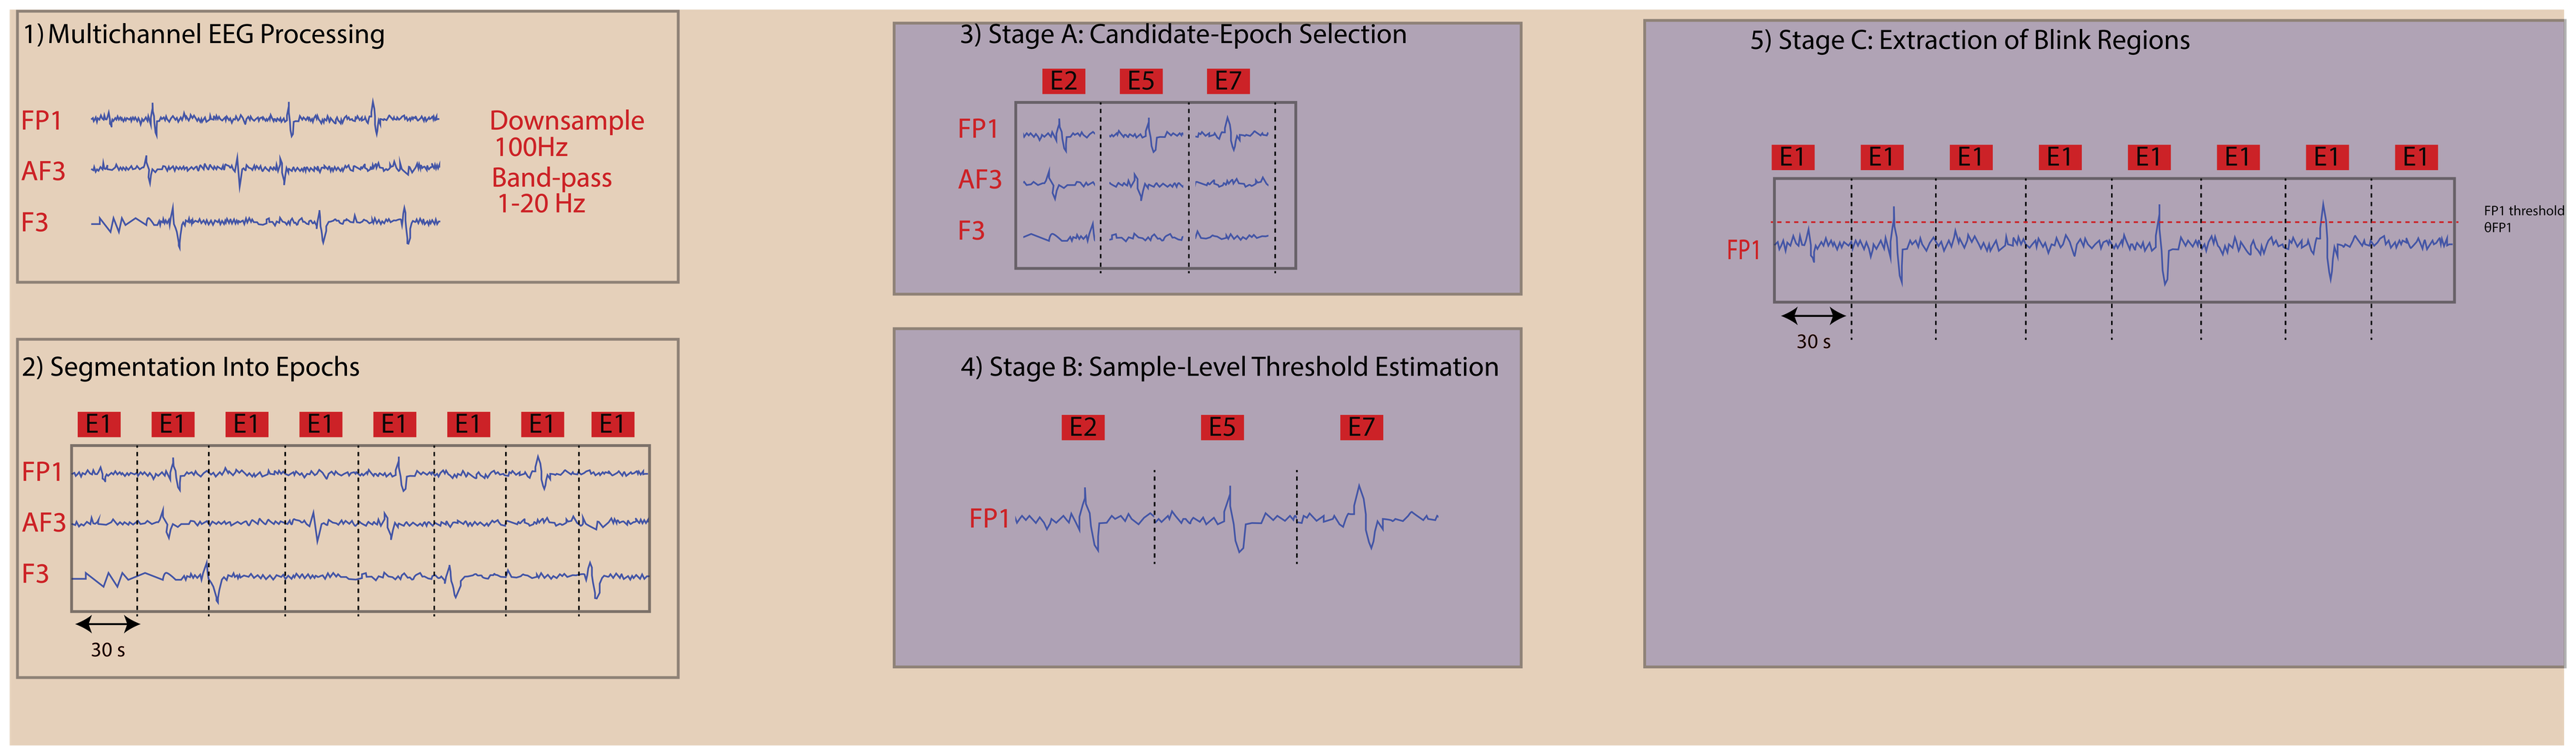
\includegraphics[width=\textwidth]{flowchart}
    \caption{
        Overview of the proposed epoch-aware pipeline for EEG blink-region detection. Continuous multichannel EEG signals are downsampled to 100 Hz, band-pass filtered from 1 to 20 Hz, and segmented into non-overlapping 30-s epochs. Stage A applies multichannel peak-to-peak screening with a union rule to select candidate epochs, represented by E2, E5, and E7 in this example. Stage B pools the samples from these candidate epochs to estimate a robust sample-level threshold independently for each channel
        , illustrated here for $FP1$.
        Stage C applies each channel's threshold to the corresponding channel across all valid epochs, including non-candidate epochs, and reports each detected blink region by its epoch, channel, onset time, and duration. Pale yellow shading denotes Stage A candidate epochs, red shading denotes detected blink regions, and dashed green lines denote the channel-specific thresholds.
    }
    \label{fig:pipeline_flow}
\end{figure*} 
\paragraph{Preprocessing}
First, the continuous recording is downsampled to a common sampling grid of \(100\)~Hz. Standardising the sampling rate makes the
amplitude thresholds and the minimum-duration gate comparable across recordings acquired on different hardware, and reduces the per-sample computational cost of the downstream stages without discarding any information needed to resolve a blink, whose
spectral content lies well below the new Nyquist frequency.
%
Second, a zero-phase band-pass filter from \(1.0\)~Hz  to \(20.0\)~Hz
is applied, \rev{which removes} slow drifts and DC offsets at the low end and high-frequency muscle and line noise at the high end, isolating the low-frequency, high-amplitude deflection that characterises an eye blink.
%
Third, each filtered recording is split into non-overlapping, fixed-length epochs.
%
\rev{Epoching enables candidate-pool selection. Rather than deriving a single threshold from the entire concatenated session, Stage~B estimates one session-specific threshold per channel from the samples pooled across the selected candidate epochs.}

\rev{In the present implementation, epoching precedes per-epoch filtering and resampling rather than the continuous-first order described above. This implementation detail is noted as a methodological limitation in Section~IV.}

 

%
\paragraph{Selection of Candidate Epochs}

The first stage, Stage~A, performs an initial epoch-level screening to identify epochs that are most likely to contain prominent blink-related activity. The screening adopts the threshold-selection approach of \citep{jas2017autoreject}, in which a peak-to-peak amplitude threshold is estimated for each channel through cross-validation. Rather than relying on a single channel, the screening decision integrates information across multiple EEG channels. An epoch is therefore selected when abnormal amplitude excursions are detected in one or more channels. At this stage, the objective is not to localize individual blink samples but to identify candidate epochs containing prominent amplitude activity. This multichannel screening strategy narrows the search space to potentially blink-related epochs for detailed sample-level analysis in the subsequent stages.




Let \(X \in \mathbb{R}^{N \times C \times T}\) denote the epoched multichannel
signal after preprocessing, where \(N\) is the number of valid epochs, \(C\) is
the number of channels, and \(T\) is the number of samples per epoch. The sample
at epoch \(i \in \mathcal{E}=\{1,\ldots,N\}\), channel
\(c \in \mathcal{C}=\{1,\ldots,C\}\), and within-epoch time index
\(t \in \{1,\ldots,T\}\) is denoted by \(x_{i,c,t}\).

For each epoch and channel, an amplitude-range statistic is computed using the  peak-to-peak value
\begin{equation}
a_{i,c}
= \max_{1 \leq t \leq T} x_{i,c,t}
- \min_{1 \leq t \leq T} x_{i,c,t}.
\end{equation}
Large values of \(a_{i,c}\) indicate that the corresponding epoch contains a high-amplitude excursion in channel \(c\), a pattern consistent with ocular or other transient artifacts.
Because signal amplitudes may vary across channels, participants, and recording conditions, a fixed peak-to-peak threshold is not imposed.
%
Instead, \rev{a channel-specific threshold \(\tau_c^\star\) is estimated from that channel's peak-to-peak amplitudes across epochs.}
Candidate thresholds are taken from the empirical range of peak-to-peak amplitudes for that channel, denoted
\(\mathcal{Q}_c=\{a_{i,c}: i \in \mathcal{E}\}\), and are evaluated by a
cross-validation criterion that measures the discrepancy between retained training epochs and validation epochs.

%
%
%



After the channel-specific thresholds, \(\tau_c^\star\), have been estimated, the peak-to-peak amplitude of each epoch is evaluated separately for each EEG channel against its corresponding threshold.
An epoch is retained as a candidate when the amplitude in at least one channel exceeds the threshold \(\tau_c^\star\) defined for that channel. Thus, the epoch-level screening decision incorporates information across multiple channels using a union rule, rather than relying on a single predefined channel. %
\rev{The set of candidate epochs is therefore}
\begin{equation}
\mathcal{B}=\{i \in \mathcal{E}: b_i=1\}.
\end{equation}


where  \(b_i\) denotes the epoch-level screening outcome indicating that epoch (i) satisfies the selection criterion. These candidate epochs represent high-amplitude segments that may contain prominent blink-related activity and are retained for subsequent sample-level blink-region detection.


 %
\paragraph{Computation of Sample-Level Blink-Region Threshold Candidates}


Stage~B estimates a sample-level amplitude threshold for each channel using samples drawn from the candidate epochs $\mathcal{B}$ identified in Stage~A.
%
\rev{Each threshold combines a measure of central tendency with a scaled robust measure of dispersion, allowing the threshold to adapt to the amplitude characteristics of each channel while limiting the influence of isolated extreme samples.
%
}


Let \(\mathcal{S}\) denote the set of epochs used for estimating the
sample-level threshold. In the primary analysis,
\(\mathcal{S}=\mathcal{B}\), so that the estimate is driven by epochs already
identified as likely to contain blink-related activity.


For each channel \(c\), all samples from the selected epochs are pooled into a
one-dimensional empirical sample set
\begin{equation}
\mathcal{Y}_c
= \{x_{i,c,t}: i \in \mathcal{S},\; 1 \leq t \leq T\}.
\end{equation}
%
%
%

The sample-level threshold is estimated using a robust location-plus-dispersion form. Let \(\xi_c\) be the channel-specific center of the sample distribution %
\rev{defined as follows:}
\begin{equation}
\xi_c = \operatorname{median}_{y \in \mathcal{Y}_c} y,
\end{equation}

%
%
%
The dispersion is estimated by the median absolute
deviation (MAD),
\begin{equation}
\operatorname{MAD}_c
= \operatorname{median}_{y \in \mathcal{Y}_c}
\left|y-\operatorname{median}_{u \in \mathcal{Y}_c}u\right|.
\end{equation}
%
%
%
%
%
\rev{The threshold candidate for channel \(c\) is then set above the channel center by a margin \(\Delta_c\),
\begin{equation}
\theta_c = \xi_c + \Delta_c .
\end{equation}
The margin \(\Delta_c\) is a fixed multiple of \(\operatorname{MAD}_c\), and the same multiple is used for every channel. A channel with a wider amplitude spread therefore receives a higher threshold.}
The set
\begin{equation}
\Theta = \{\theta_c: c \in \mathcal{C}\}
\end{equation}
constitutes the channel-wise threshold candidates passed to the blink-region extraction stage.
 %
\paragraph{Extraction of Blink Regions}
The final stage, stage C, applies the sample-level thresholds
\(\Theta=\{\theta_c\}_{c=1}^{C}\) obtained in Stage~B to obtain channel-wise
blink regions. Specifically, blink regions are searched for within each valid
epoch \(i \in \mathcal{E}=\{1,\ldots,N\}\) and each channel
\(c \in \mathcal{C}\), by comparing the samples \(x_{i,c,t}\) of that epoch and
channel against the threshold candidate \(\theta_c\) of the same channel.
The final output of this stage is therefore a channel-indexed collection of blink regions, each represented by an epoch identifier, a channel label, an onset time, and duration.

%

 
%


\subsection{Experimental Setup}
\label{sec:exp_setup}


\subsubsection{Datasets}
\label{sec:datasets}
%
Two EEG corpora acquired during sustained simulated-driving tasks were used. The corpora differed in their acquisition montages and data provenance, allowing the proposed method to be evaluated under different hardware setups.

The public corpus contains data from 27 participants who performed an approximately 90-minute lane-keeping task in an immersive driving simulator~\citep{cao2019multichannel}, and is referred to as Cao2018 henceforth. The Cao2018 corpus is publicly available under a Creative Commons Attribution 4.0 International licence~\citep{cao2019multichannel} and was accessed via the published figshare repository (DOI: 10.6084/m9.figshare.6427334.v5). This study used the raw recordings. All 32 recorded electrophysiological channels (30 scalp electrodes and the A1/A2 mastoid reference channels) were supplied to the pipeline. These 32 channels were Fp1, F3, Fp2, F4, FT7, FC3, C3, FC4, FT8, C4, TP7, CP3, TP8, CP4, T5, P3, O1, T6, P4, O2, F7, T3, Fz, FCz, Cz, Pz, Oz, F8, T4, CPz, A1, and A2.

The Internal corpus is a dataset collected in house, comprising data from 17 participants, recorded during a simulated lane-keeping task. The Internal corpus was collected under a protocol approved by the Human Research Ethics Committee of Universiti Pendidikan Sultan Idris (Sultan Idris Education University; reference number 2021-0290-01). All participants provided written informed consent before the recording session. EEG was acquired with a 128-channel EGI HydroCel system, with CPz as the reference. Although the original recordings used a high-density montage, the present analyses retained a predefined subset of 32 electrodes corresponding to conventional 10--20 scalp locations, following the subsampled 128-to-32-channel montage of~\citep{Hatlestad_2023_reliable}. The 32 channels are Fp1, AF3, F3, Fp2, AF4, F4, FC5, FC1, C3, FC2, FC6, C4, CP5, CP1, CP2, CP6, \rev{P8}, P3, PO3, O1, PO4, P4, P7, O2, F7, T7, Fz, Cz, Pz, Oz, F8, and T8.

We divided the 32 electrodes into four anatomical regions (frontal, central, parietal, and occipital) and further divided each region into left and right hemispheres, as per~\citep{black2012}, as shown in Figure~\ref{fig:eeg_map}. In the figure, the resulting eight regions (frontal left, frontal right, central left, central right, parietal left, parietal right, occipital left, and occipital right) are abbreviated FL, FR, CL, CR, PL, PR, OL, and OR, respectively. The figure shows the scalp locations of the 32 electrodes with the blue circles represent electrodes located in both the Internal and Cao2018 montages, the yellow circles represent electrodes located only in the Internal montage, and the red circles represent electrodes located only in the Cao2018 montage.



\begin{figure}[ht]
    \centering
    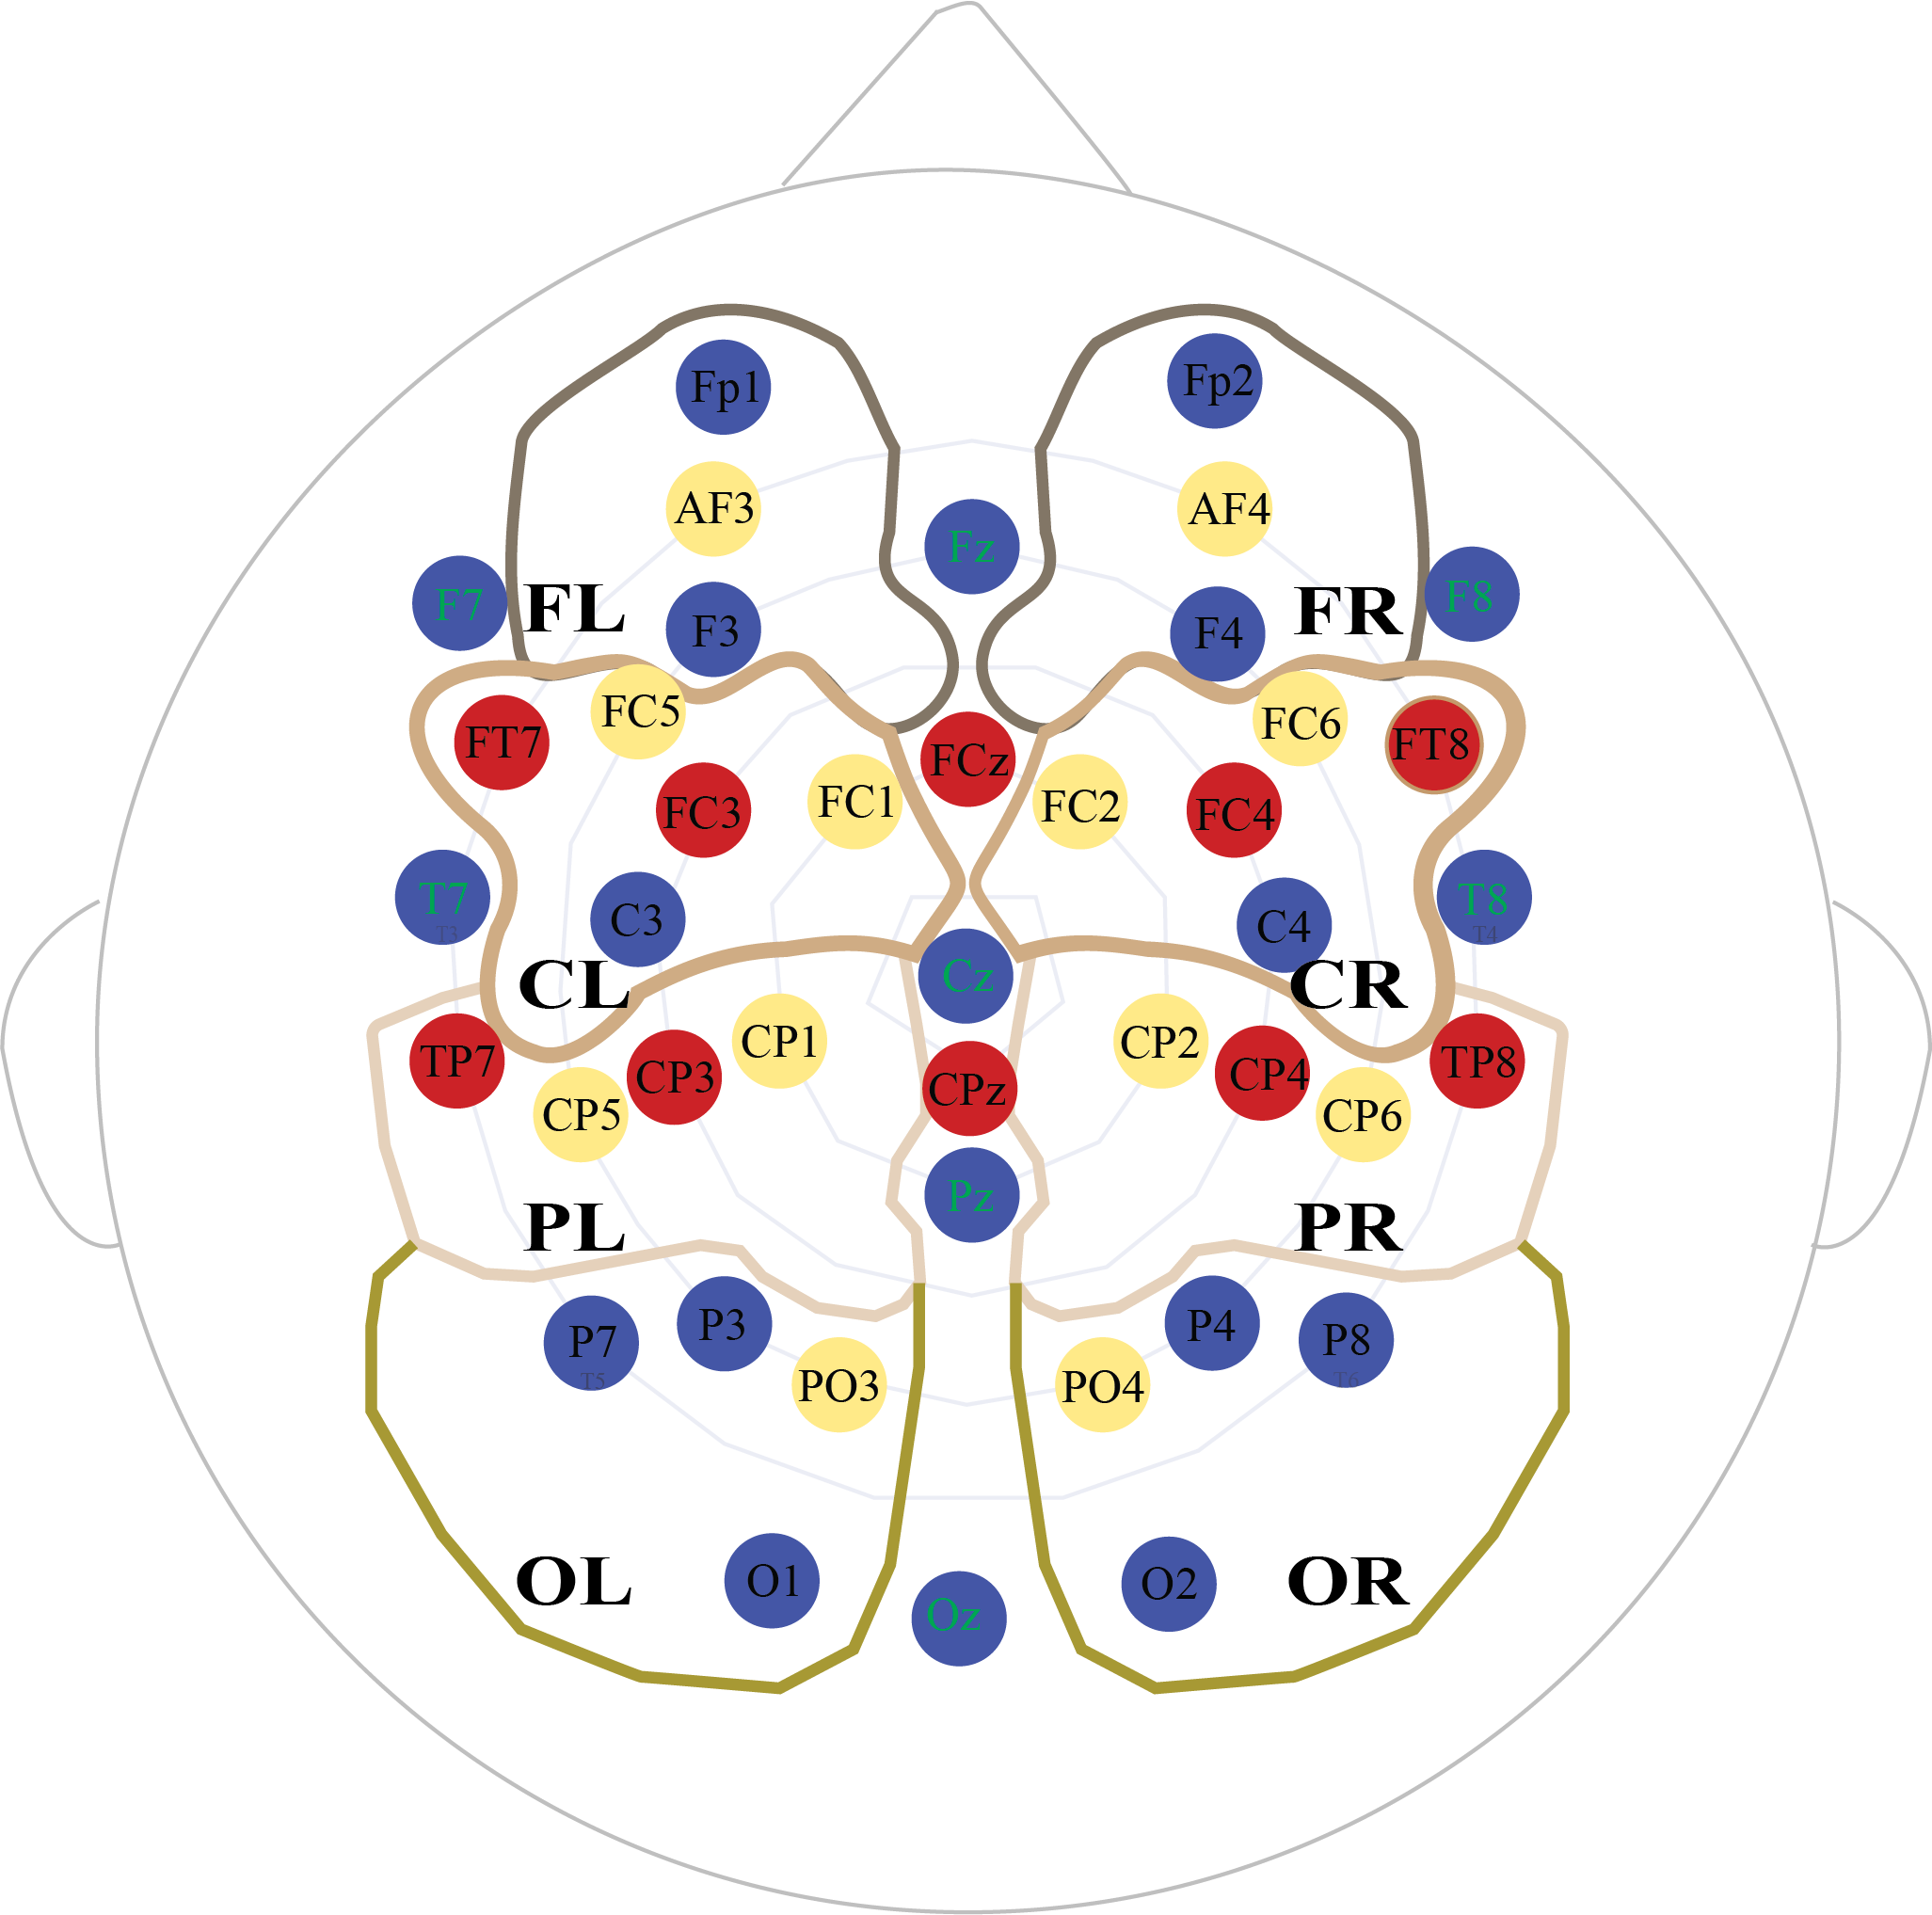
\includegraphics[width=0.9\linewidth]{eeg_map}
    \caption{Scalp locations of the 32 electrodes used in this study, divided into eight anatomical regions (frontal left/right, central left/right, parietal left/right, and occipital left/right, abbreviated FL, FR, CL, CR, PL, PR, OL, and OR). Blue circles mark electrodes present in both the Internal and Cao2018 montages, yellow circles mark electrodes present only in the Internal montage, and red circles mark electrodes present only in the Cao2018 montage.}
    \label{fig:eeg_map}
\end{figure}

 
\subsubsection{Ground-Truth Annotation}
\label{sec:annotation}
%


Reference blink events for both corpora were established by manual annotation. Two raters, blinded to the study objectives and to the outputs of the blink-detection algorithms evaluated in this study, annotated the recordings, and each blink was marked as an interval delimited by its onset and offset. The first rater identified the blinks in each recording and marked their onsets and offsets. The second rater then reviewed every recording independently, checking the onset and offset of each marked interval and searching the recording for blinks that had been missed or events that had been marked incorrectly. Discrepant annotations were reviewed jointly and resolved by consensus, and the consensus labels served as the reference for all evaluations. Because the second rater reviewed the first rater's annotations rather than producing a separate annotation from scratch, no inter-rater agreement statistic was computed. A recording entered the analysis only after its annotation had been marked as complete.

\paragraph{Internal corpus.}
For the Internal corpus, a face video recorded in synchrony with the EEG served as the primary behavioural reference. The video was captured by a USB webcam at 30 frames/s and a resolution of $1280\times720$ pixels.
%
Annotation relied on three time-aligned sources, namely the video itself, a vertical electrooculographic (EOG) derivation, and an eye aspect ratio (EAR) trace computed from facial landmarks in each video frame~\citep{soukupova2016realtime}. The EAR quantifies eye opening, falling as the eyelids close and recovering as they reopen. An event was accepted as a blink only when a closing and reopening of the eyelids was visible in the video. Blink onset was placed where the eyelids began to close and the EAR began to fall from its open-eye level, and blink offset where the eyelids had returned to the open position and the EAR had recovered. Each boundary was then checked against the characteristic high-amplitude blink transient in the vertical EOG~\citep{croft2000removal}. The video and EAR thus determined whether an event was a blink and where it began and ended, whereas the vertical EOG provided an electrophysiological check on that timing. All marked events, whether the eyelid closure was complete or partial, were treated as reference blinks in the evaluation.

\paragraph{Cao2018 corpus.}
No video recordings or separate EOG channels are distributed with the Cao2018 corpus. Its event markers describe only the driving task, namely lane-departure onsets and the onsets and offsets of the driver's corrective responses, and no blink annotations are provided~\citep{cao2019multichannel}. Blinks in this corpus were therefore annotated from the EEG alone. The raters inspected each recording with Fp1 and Fp2 displayed by default and the remaining channels available on demand. They marked as blinks the transient, high-amplitude deflections ~\citep{iwasaki2005effects,croft2000removal,kleifges2017blinker}. Blink onset was placed where this deflection departed from the preceding baseline, and blink offset where it returned to baseline.
%
 
\subsubsection{Evaluation Metrics}
\label{sec:metrics}
%



\paragraph{Event matching.}
Performance was evaluated at the blink-event level rather than at the sample level. For a predicted interval $P$ and a reference interval $G$, temporal
overlap was quantified using intersection over union (IoU)~\cite{Startsev2023}:
\begin{equation}
    \operatorname{IoU}(P,G)
    = \frac{|P \cap G|}{|P \cup G|}.
\end{equation}
Here, $|\cdot|$ denotes interval duration.
A predicted interval was eligible for a match when its IoU with an unmatched reference interval was at least 0.1. \rev{The IoU threshold of 0.1 was chosen to ensure event-level correspondence while accommodating the onset and offset variability inherent in manual EEG annotation. This threshold verifies that predicted and reference events overlap in time without requiring precise boundary alignment.} Matching was one-to-one, so a predicted or reference interval could contribute to at most one match.

%

\paragraph{Session-level measures.}
Precision, recall, and $F_1$ were calculated independently for each session $s$ from the event counts:
\begin{align}
    \operatorname{Precision}_s
        &= \frac{\mathrm{TP}_s}{\mathrm{TP}_s+\mathrm{FP}_s}, \\
    \operatorname{Recall}_s
        &= \frac{\mathrm{TP}_s}{\mathrm{TP}_s+\mathrm{FN}_s}, \\
    F_{1,s}
        &= \frac{2\,\operatorname{Precision}_s\operatorname{Recall}_s}
        {\operatorname{Precision}_s+\operatorname{Recall}_s}.
\end{align}

\paragraph{Macro-averaging.}
For a measure $M\in\{\operatorname{Precision},\operatorname{Recall},F_1\}$,
the reported macro-average over $S$ sessions was
\begin{equation}
    \overline{M}=\frac{1}{S}\sum_{s=1}^{S}M_s.
\end{equation}
Thus, each session contributed equally, irrespective of its number of annotated  blinks. This approach prevents sessions with many blinks from dominating the headline result, as would occur with micro-averaging.
 
\subsubsection{Code Availability}
\label{sec:code_availability}
%
\rev{To support reproducibility, the source code for the proposed pipeline, the baseline implementations, and the scripts used to run all experiments reported in this paper are publicly available at \url{https://github.com/pyresearchs/double_thresholding_blink}.}
 
%
%
%





  %
\section{Results}
\label{sec:results}



%
%
%
\subsection{Experiment 1: EEG Channel-Subset Analysis}
\label{sec:exp1_channel}
%



%
%
%
%
%
%
%
%
%
%
%

In the proposed pipeline, Stage~A screens epochs using a union rule over the channels supplied to the pipeline, so changing the channel set can also change which epochs reach Stage~B. Restricting the input channels therefore changes the detector itself, not merely the signals presented to a fixed detector. The EEG channel-subset analysis accounts for this coupling by re-running the complete pipeline separately for each channel subset. We first supply the complete 32-channel montage to the pipeline as a baseline, reported in Section~\ref{sec:exp1_reference}. This configuration assumes no prior knowledge of which brain region projects blinks most strongly, making it the most general reference for the reduced configurations that follow.
%
Section~\ref{sec:exp1_regional} then evaluates anatomically defined regional subsets, where the union rule operates only over the channels within each region. Comparing these subsets with the full montage identifies which scalp regions yield the strongest detection performance within the pipeline and quantifies how performance changes when the remaining regions are excluded.
%
Section~\ref{sec:exp1_single_channel} takes the reduction further by supplying one electrode at a time, so that the union rule reduces to single-channel screening and both the candidate epochs and the threshold are derived from that electrode alone. Comparison with the full montage then shows whether a single electrode can retain comparable detection performance, which would support a simpler and more practical single-channel system. 
%
\subsubsection{Full-Montage Reference}
\label{sec:exp1_reference}

%
\paragraph{Per-Electrode Detection}
\label{sec:exp1_per_electrode}

%
Figure~\ref{fig:exp1_full_montage_per_electrode} shows the per-electrode detection performance obtained when all 32 channels were supplied to the pipeline. On both datasets, detection quality was highest at Fp1 and Fp2 rather than uniform across the frontal region. On Internal, Fp2 and Fp1 reached $F_1$ values of 86.82\% and 86.32\%, respectively. Performance fell at the neighbouring sites AF4 and AF3 to 80.32\% and 73.76\% and dropped further at F3 and F4 to 45.65\% and 45.23\%. On Cao2018, Fp1 and Fp2 reached $F_1$ values of 79.68\% and 78.45\%, respectively, whereas F3 and F4 were lower at 59.51\% and 57.99\%.
 
%
The central electrodes showed a dataset-specific asymmetry. On Internal, C3 reached an $F_1$ of 61.06\% while C4 reached only 1.85\%. On Cao2018, C3 and C4 performed similarly at 31.08\% and 30.18\%, indicating that the pronounced C3--C4 asymmetry was specific to Internal.
 
%
The parietal and occipital electrodes performed markedly worse than the frontal and central electrodes, and their performance differed between datasets. On Internal, the four parietal electrodes, CP1, CP2, CP5 and CP6, were uniformly near floor, with $F_1$ values between 1.75\% and 2.19\%. The eight occipital electrodes, P7, P3, PO3, O1, PO4, O2, P4 and P8, showed slightly more spread, from 1.77\% at P4 to 3.60\% at PO3. On Cao2018, the two parietal electrodes were more informative but remained well below the frontal and central regions, with CP3 and CP4 reaching 17.84\% and 19.56\%. The Cao2018 occipital region was also more heterogeneous than its Internal counterpart. P3 and P4 scored highest at 12.80\% and 12.67\%, T5 and T6 were intermediate at 9.26\% and 8.30\%, and O1 and O2 were near floor at 3.10\% and 3.33\%.

\begin{figure}[ht]
    \centering
    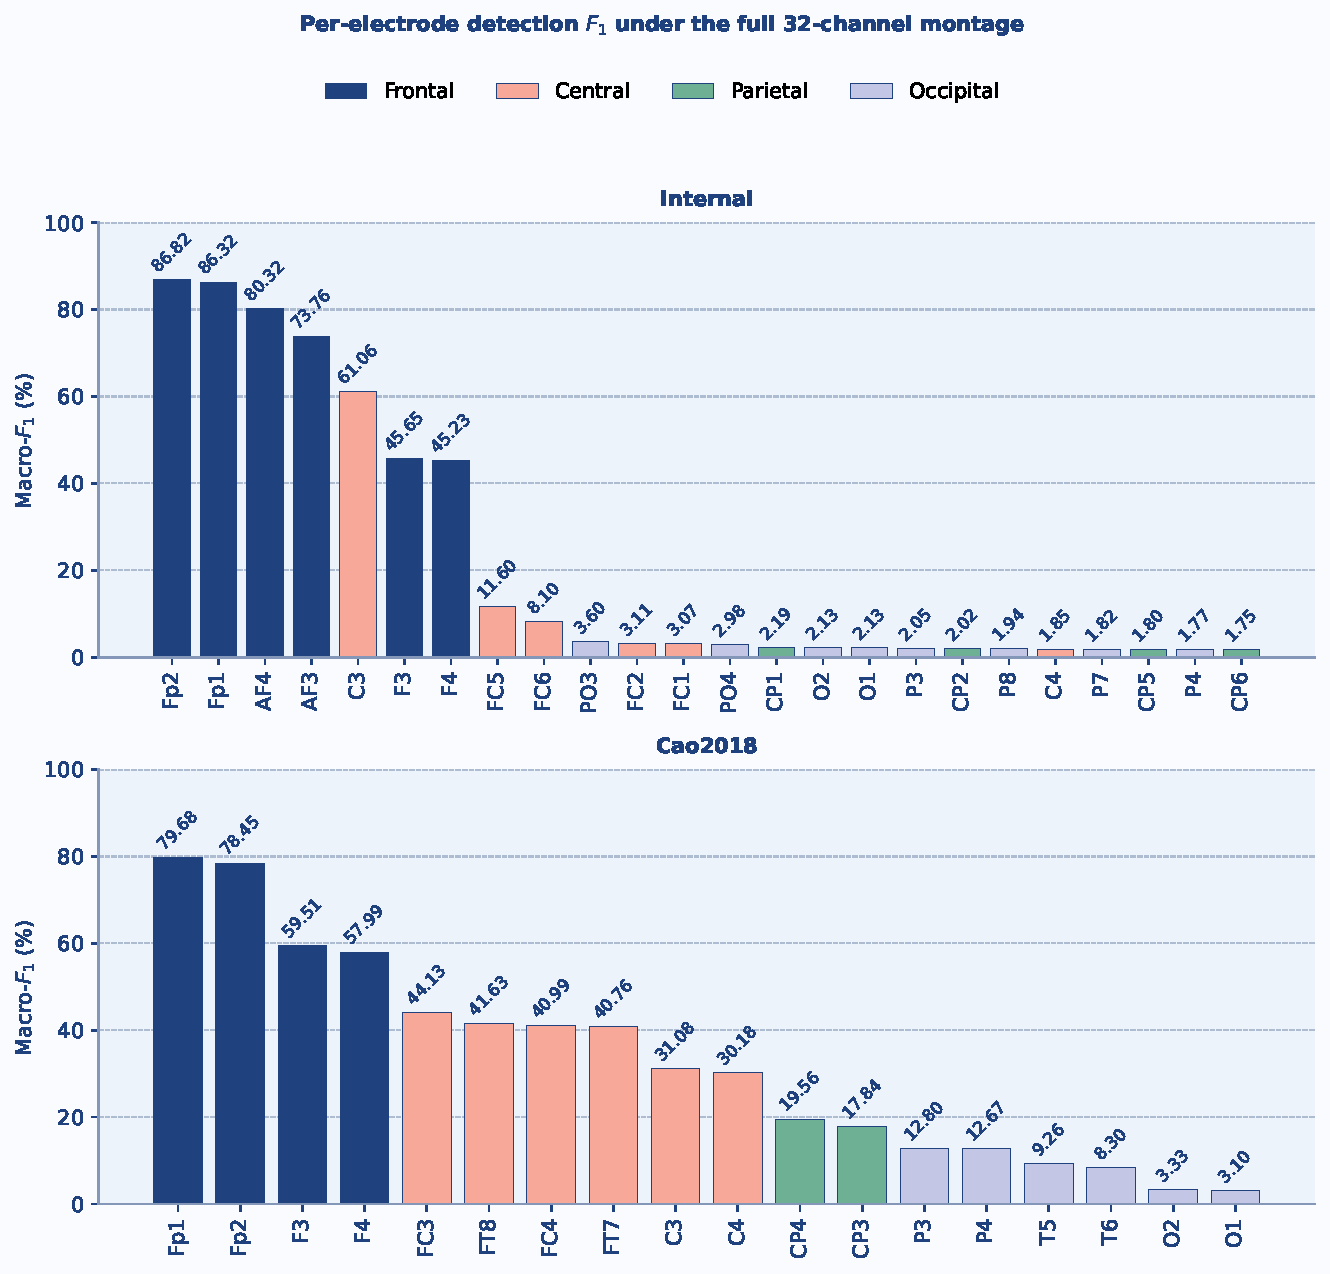
\includegraphics[width=0.9\linewidth]{fig_exp1_full_montage_per_electrode.pdf}
    \caption{Per-electrode detection $F_1$ for every electrode in the four curated
        anatomical regions, scored in the full-montage run, coloured by scalp region. Each bar is one electrode's session-mean $F_1$
        under the complete pipeline using all 32 channels.
%
%
%
%
%
%
%
    }
    \label{fig:exp1_full_montage_per_electrode}
\end{figure}
 



%
\subsubsection{Regional Channel Subsets}
\label{sec:exp1_regional}

%
\paragraph{Per-Electrode Detection}
\label{sec:exp1_regional_per_electrode}

%
The full-montage analysis above established the per-electrode detection performance when all 32 channels were supplied to the pipeline. The present analysis reduces the input to anatomically defined regions and asks how each region performs as a self-contained detector. For each of the four regions, frontal, central, parietal, and occipital, the complete pipeline from Stage~A to Stage~C was rerun using only the electrodes within that region. The 30-s epochs, preprocessing, and thresholding parameters were identical to those of the full-montage reference. With a regional input, the Stage~A union rule operates only over the channels within that region, so the candidate epochs, and therefore the channel-specific thresholds estimated from them, are determined by that region alone. Results are reported per electrode, but each electrode's score is obtained from the rerun of its own region.
%
 
%
As shown in Figure~\ref{fig:exp1_subset_per_electrode}, per-electrode detection quality within the regional reruns was highest at Fp1, Fp2 and the neighbouring frontal electrodes rather than uniform across the frontal region.
On Internal, Fp2, Fp1, AF4 and AF3 were the four strongest electrodes in the frontal regional rerun, at 85.28\%, 84.84\%, 77.04\% and 70.70\%, respectively, and performance then fell sharply at F3 and F4 to $42.68\%$ and $41.00\%$. On Cao2018, the frontal region consists of Fp1, Fp2, F3 and F4 only, which reached 78.80\%, 77.05\%, 55.97\% and 54.64\%, respectively.
Every one of these frontal electrodes scored lower in the regional rerun than in the full-montage run (Section~\ref{sec:exp1_reference}), but restricting Stage~A and Stage~B to the frontal electrodes left their ranking by $F_1$ unchanged in both datasets.
%
The central regional rerun again showed a dataset-specific asymmetry. On Internal, C3 reached an $F_1$ of $58.59\%$ while C4 reached only $1.73\%$, so the pronounced C3--C4 asymmetry seen in the full-montage run persisted. On Cao2018, in contrast, C3 and C4 remained close together at $27.67\%$ and $26.62\%$, respectively, so the asymmetry again stayed specific to Internal. Parietal and occipital electrodes scored much lower in their regional reruns. The best parietal electrode reached only $1.92\%$ on Internal (CP1) and $15.63\%$ on Cao2018 (CP4). The best occipital electrode reached $3.35\%$ on Internal (PO3) and $10.04\%$ on Cao2018 (P3). Overall, the regional reruns preserved the pattern observed in the full-montage run, with $F_1$ highest at Fp1, Fp2 and the neighbouring frontal electrodes and lower at most central, parietal and occipital electrodes.

\begin{figure}[ht]
    \centering
    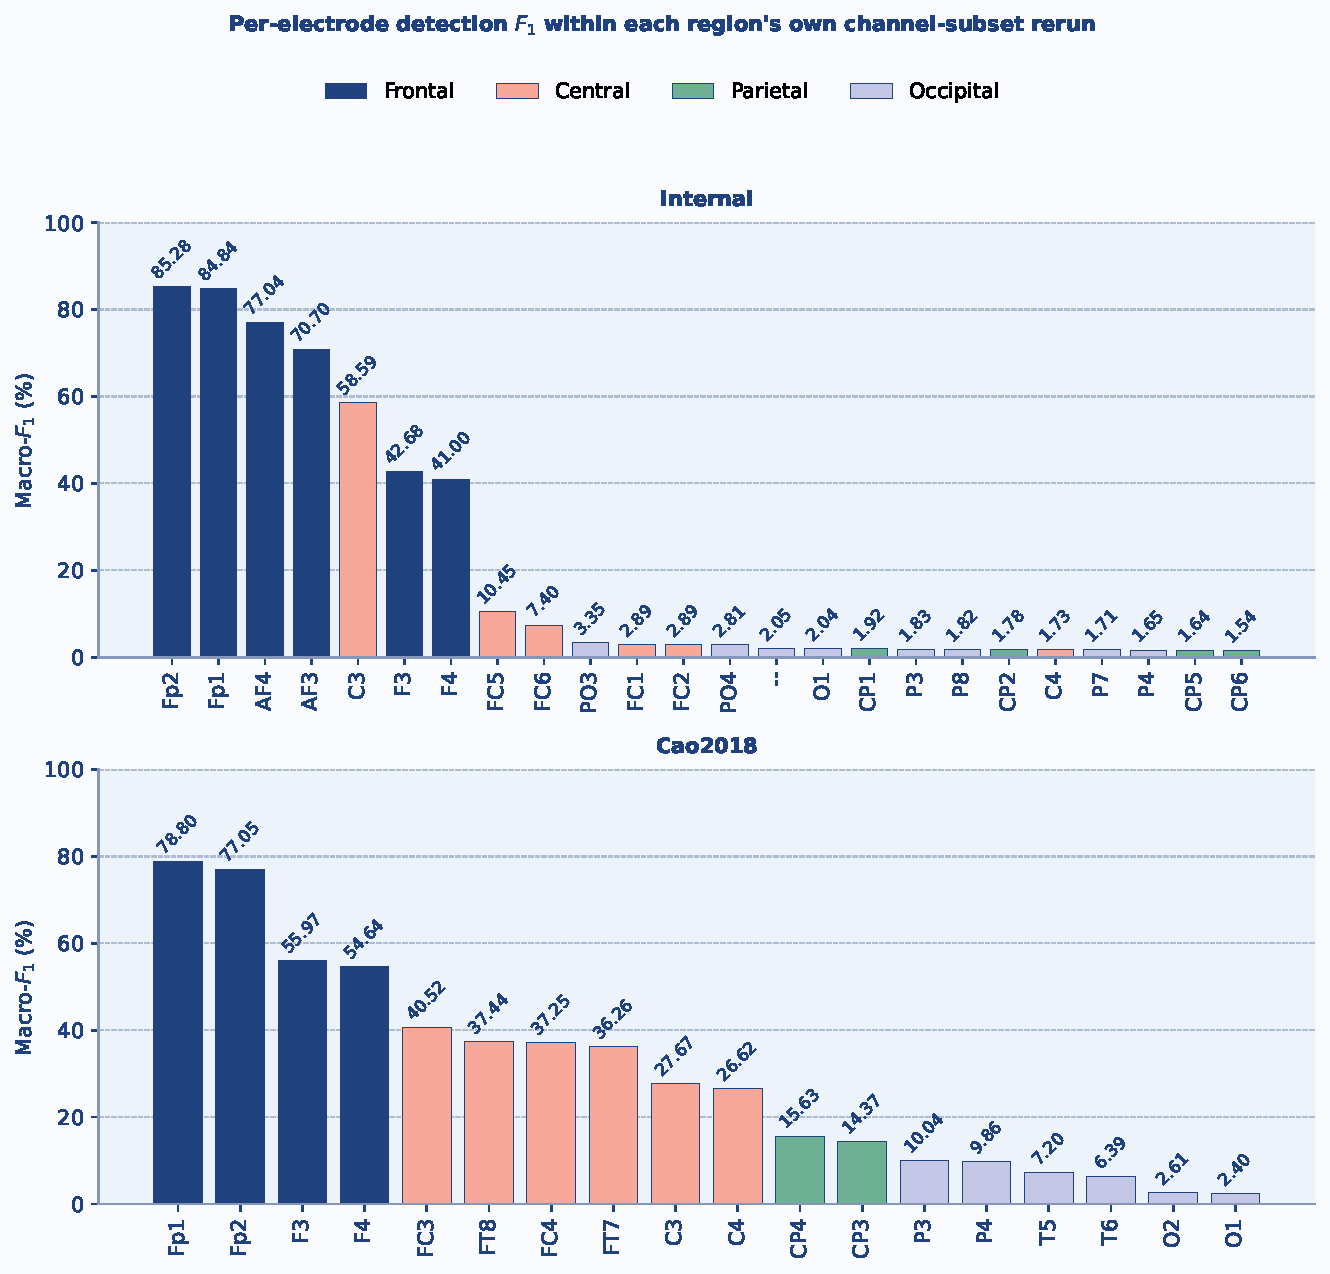
\includegraphics[width=0.9\linewidth]{fig_exp1_subset_per_electrode.pdf}
    \caption{Per-electrode detection $F_1$ in the regional rerun of each electrode's own region, coloured by region. Each bar is one electrode's session-mean $F_1$ when only the electrodes of its region were supplied to the pipeline.}
    \label{fig:exp1_subset_per_electrode}
\end{figure}
 
%
\paragraph{Electrode-Level Significance Testing}
\label{sec:exp1_regional_electrode_level_stats}

%
The descriptive differences between the regional reruns and the full-montage reference were next tested for every electrode using session-paired comparisons. For each electrode in the four anatomical subsets shown in Figure~\ref{fig:eeg_map}, its session-level $F_1$ in the rerun of its own region was paired with its session-level $F_1$ in the full-montage run, using the sessions common to both. For example, the $F_1$ of Fp1 when the pipeline was run on the frontal electrodes only was compared with the $F_1$ of Fp1 when all 32 channels were supplied to the pipeline, and the same comparison was made for every other electrode within its own region. Each electrode was tested with a two-tailed Wilcoxon signed-rank test paired by session, with $p$-values Bonferroni-corrected over the electrodes tested within each dataset. Figure~\ref{fig:exp1_subset_per_electrode_stats} shows, for every electrode, its session-mean $F_1$ in the regional rerun overlaid on its session-mean $F_1$ in the full-montage run, with an asterisk marking electrodes that were significant after correction.
 
%
On Internal (Figure~\ref{fig:exp1_subset_per_electrode_stats}A), all 24 electrodes had a lower session-mean $F_1$ in the regional rerun than in the full-montage run, and the reduction was significant after correction for 11 of them (adjusted $p < 0.05$). Fp2 and Fp1 had the two highest regional-rerun scores, but neither differed significantly from the full-montage run (adjusted $p > 0.05$ for both). In contrast, AF4 and AF3, the third- and fourth-highest-performing electrodes, were significantly lower in the regional rerun, as were F3 and F4. In the central region, the reduction was significant for C3 and FC6 but not for FC5, FC1, FC2 or C4. In the parietal region, it was significant for CP2, CP5 and CP6 but not for CP1. In the occipital region, as defined in Figure~\ref{fig:eeg_map}, only PO3 and PO4 were significantly lower, and O1, O2,P3, P8, P7 and P4 were not. Three electrodes, CP2, CP5 and FC5, lay close to the corrected threshold. Table~\ref{tab:app_regional_internal} in Appendix~\ref{app:per_electrode_stats} gives their exact adjusted $p$-values, together with the session-mean $F_1$ and $\Delta F_1$ of every electrode.
 
%
On Cao2018 (Figure~\ref{fig:exp1_subset_per_electrode_stats}B), all 18 electrodes likewise scored lower in the regional rerun than in the full-montage run, but significant reductions were far more widespread than on Internal. Sixteen of the 18 reductions were significant after correction (adjusted $p < 0.05$). As on Internal, only Fp1 and Fp2 did not reach significance (adjusted $p > 0.05$ for both), whereas F3 and F4, the third- and fourth-highest-performing electrodes, did. Unlike on Internal, the reduction was significant at all six central electrodes, including both C3 and C4, and at both parietal electrodes, CP3 and CP4. It was also significant at all six occipital electrodes, as defined in Figure~\ref{fig:eeg_map}. Table~\ref{tab:app_regional_cao2018} in Appendix~\ref{app:per_electrode_stats} lists the session-mean $F_1$, $\Delta F_1$ and adjusted $p$-value for every electrode.
 
%

\begin{figure}[ht]
    \centering
    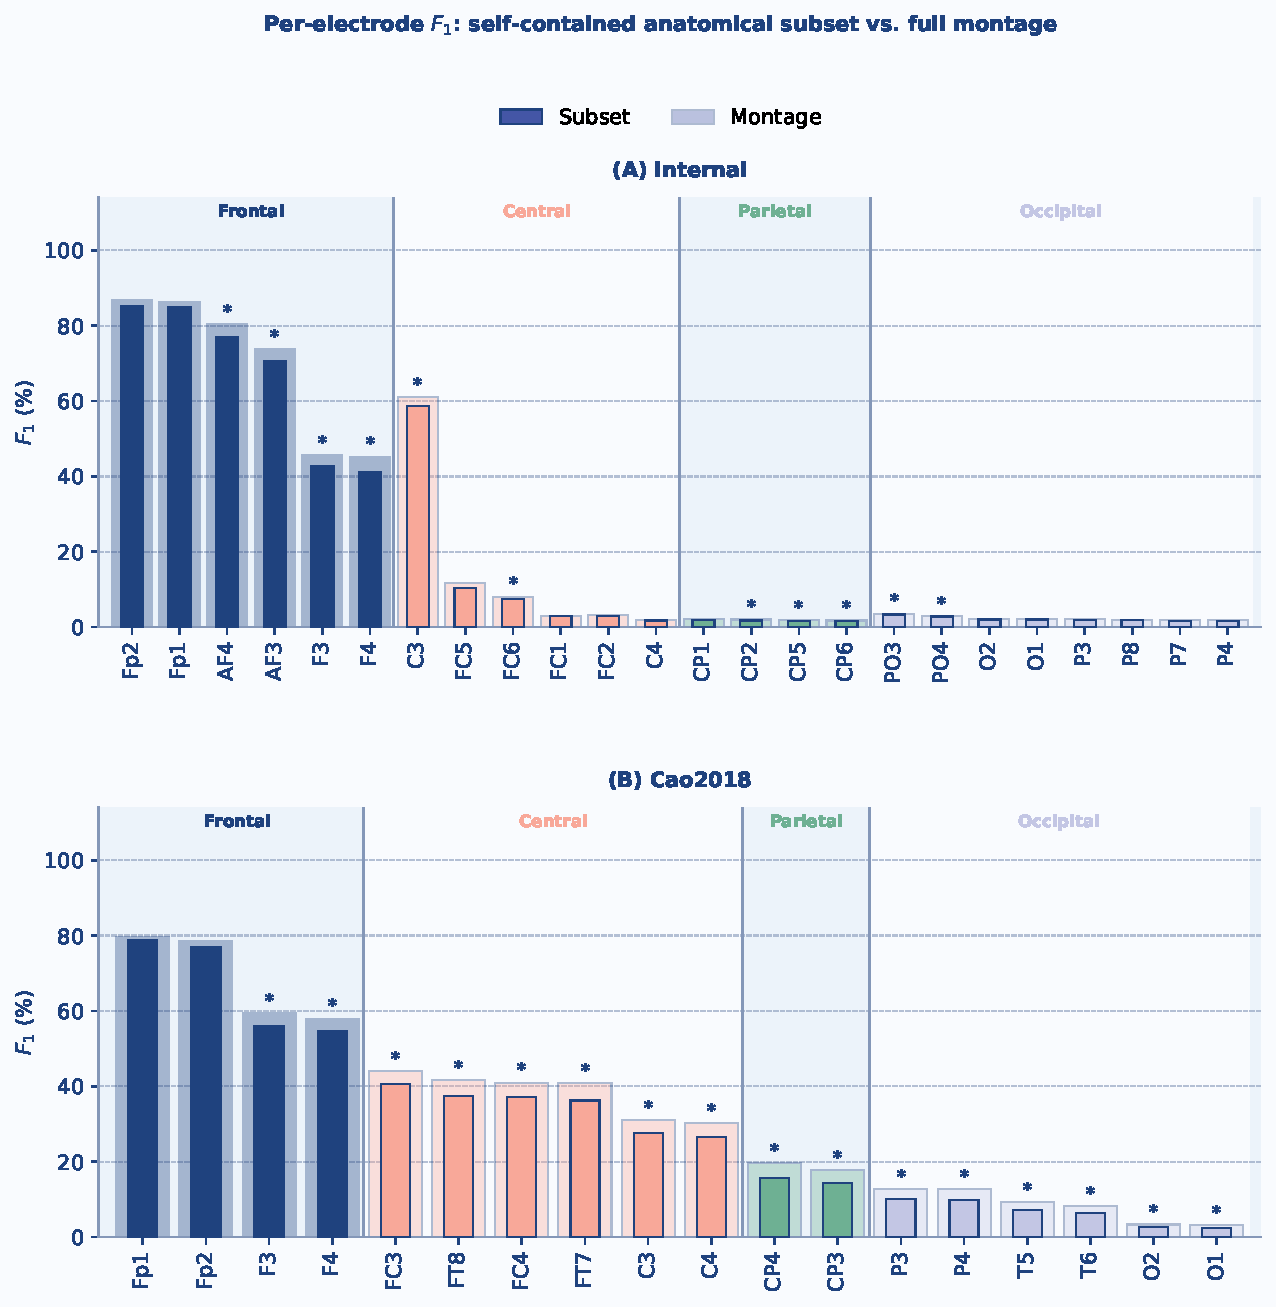
\includegraphics[width=\linewidth]{fig_exp1_subset_per_electrode_stats.pdf}
    \caption{Per-electrode comparison of $F_1$ for each electrode in the rerun of its own anatomical region (narrow, opaque bars) and in the full-montage run (wide, translucent bars), for (A)~Internal and (B)~Cao2018. Bars show session-mean $F_1$. Electrodes are grouped by the anatomical regions in Figure~\ref{fig:eeg_map} and ordered by descending regional-rerun $F_1$ within each region. Comparisons are paired by session using two-tailed Wilcoxon signed-rank tests, with $p$-values Bonferroni-corrected separately over the electrodes tested within each dataset. An asterisk marks adjusted $p < 0.05$.}
    \label{fig:exp1_subset_per_electrode_stats}
\end{figure}

%
%
%
%
%
%
%
%
%
%
%



%
%
%


%
%
%
%
%

%
%
%
%
%
%
%



\begin{figure}[ht]
    \centering
    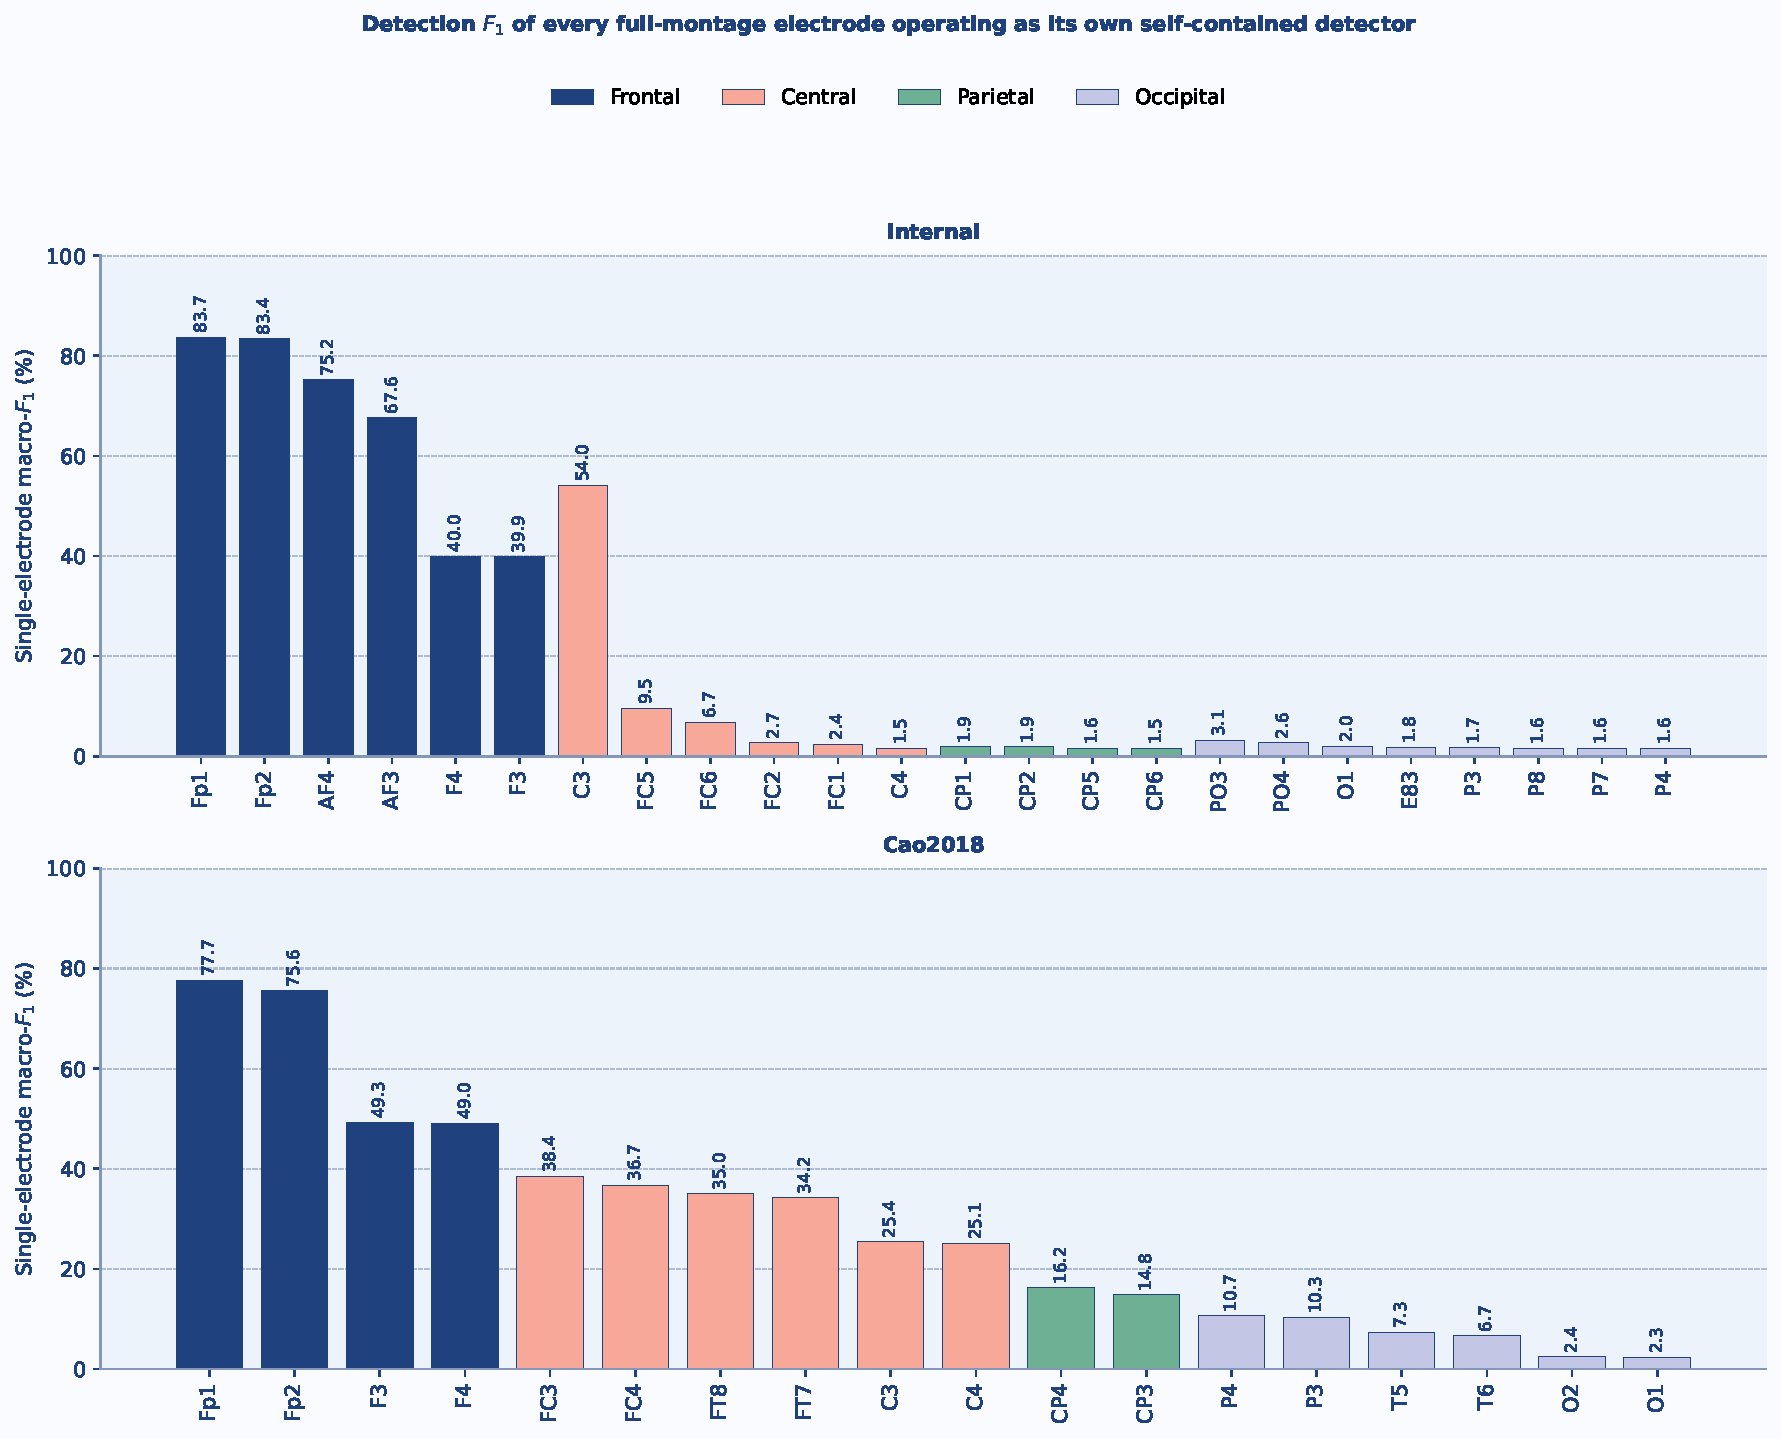
\includegraphics[width=0.9\linewidth]{fig_exp1_single_channel_boxplot.pdf}
    \caption{Detection $F_1$ of every electrode in the four curated anatomical regions
    operating as its own self-contained detector, in which the complete Stage~A--Stage~C pipeline was rerun on that one
    electrode alone, coloured by scalp region.}
    \label{fig:exp1_single_channel}
\end{figure}

\subsubsection{Single-Channel Operation}
\label{sec:exp1_single_channel}

%
The regional analysis above examined how anatomical subsets of the montage performed as self-contained detectors. The present analysis takes this reduction one step further and asks whether each electrode can independently support the complete proposed detector. For every electrode in the four anatomical regions, the complete pipeline from Stage~A to Stage~C was rerun using that electrode alone, giving 24 single-electrode detectors on Internal and 18 on Cao2018. The 30-s epochs, preprocessing, and thresholding parameters were identical to those of the full-montage reference. With a single input channel, the Stage~A union rule reduces to single-channel screening, so both the candidate epochs and the threshold are derived from that electrode alone. Each electrode's score therefore reflects a self-contained single-electrode detector. 
%
\paragraph{Per-Electrode Detection}
\label{sec:exp1_single_channel_per_electrode}

%
Ranked by mean single-electrode macro $F_1$, Fp1, Fp2, AF4 and AF3 topped Internal's ranking at 83.73\%, 83.37\%, 75.16\% and 67.59\%, respectively (Figure~\ref{fig:exp1_single_channel_stats}; Figure~\ref{fig:exp1_single_channel}). These are the same four frontal electrodes identified by the regional analysis, and in the same order except that Fp1 now leads Fp2 by 0.36 percentage points rather than trailing it. C3 came next with an $F_1$ of $54.05\%$, ahead of the remaining two canonical frontal electrodes, F4 and F3, at $39.98\%$ and $39.85\%$. Performance then fell sharply across the remaining 17 electrodes, with every parietal and occipital electrode below $3.2\%$ and C4 the weakest overall at $1.51\%$.
 
%
On Cao2018, Fp1, Fp2, F3 and F4 topped the single-electrode ranking at 77.65\%, 75.59\%, 49.30\% and 49.03\%, respectively, matching both the identity and the order of the full-montage ranking (Figure~\ref{fig:exp1_single_channel_stats}). Performance then dropped to $38.44\%$ at FC3, the first of the six central electrodes that occupied the next six places. FC4, FT8 and FT7 followed at 36.72\%, 34.99\% and 34.22\%, respectively, and C3 and C4 were the weakest central electrodes at $25.43\%$ and $25.10\%$. Performance declined further at the parietal electrodes, which ranged from $14.80$ to $16.22\%$. It declined again at the occipital electrodes, where O1 was the weakest electrode overall at $2.28\%$. This confirms, within the four declared regions, the same decline from the frontal to the occipital region seen in the full-montage run and the regional analysis (Sections~\ref{sec:exp1_reference} and~\ref{sec:exp1_regional}).
 
%



\paragraph{Electrode-Level Significance Testing}
\label{sec:exp1_single_channel_electrode_level_stats}

%
The descriptive differences between single-electrode and full-montage operation were next tested for every electrode using session-paired comparisons. For each electrode, its session-level $F_1$ when used as the only input channel was paired with its session-level $F_1$ in the full-montage run, using the sessions common to both. For example, the $F_1$ of Fp2 when the pipeline was run on Fp2 alone was compared with the $F_1$ of Fp2 when all 32 channels were supplied to the pipeline, and the same comparison was made for every other electrode.
%
Each electrode was tested with a two-tailed Wilcoxon signed-rank test paired by session, and $p$-values were Bonferroni-corrected over the electrodes tested within each dataset.
Figure~\ref{fig:exp1_single_channel_stats} shows, for every electrode, its session-mean $F_1$ operating alone overlaid on the same electrode's session-mean $F_1$ under the full montage, with an asterisk marking electrodes that were significant after correction.
 
%
On Internal (Figure~\ref{fig:exp1_single_channel_stats}A), every electrode scored lower in the single-electrode run than in the full-montage run, with $\Delta F_1$ ranging from $-7.02$ percentage points at C3 to $-0.15$ percentage points at CP2. These reductions were significant after correction for 14 of the 24 electrodes (adjusted $p < 0.05$). Fp1 and Fp2 retained the two highest single-electrode scores, and neither differed significantly from the full-montage run (adjusted $p > 0.05$ for both). In contrast, the other four frontal electrodes, AF4, AF3, F4 and F3, were all significantly lower. In the central region, the reduction was significant for C3, FC5 and C4 but not for FC6, FC2 or FC1. In the parietal region, only CP1 was significantly lower, whereas CP2, CP5 and CP6 were not. In the occipital region, as defined in Figure~\ref{fig:eeg_map}, the reduction was significant for PO3, PO4, O2, P3, P8 and P7, leaving O1 and P4 as the only exceptions. Table~\ref{tab:app_single_internal} in Appendix~\ref{app:per_electrode_stats} lists the session-mean $F_1$, $\Delta F_1$ and adjusted $p$-value for every electrode.
 %
On Cao2018 (Figure~\ref{fig:exp1_single_channel_stats}B), all 18 electrodes likewise scored lower in the single-electrode run than in the full-montage run, and 16 of these reductions were significant after correction (adjusted $p < 0.05$). As on Internal, only Fp1 and Fp2 did not reach significance (adjusted $p > 0.05$ for both). F3 and F4, which had the third- and fourth-highest single-electrode scores, showed the two largest reductions ($\Delta F_1 = -10.21$ and $-8.96$ percentage points, respectively). The reduction was also significant at all six central electrodes, including both C3 and C4, and at both parietal electrodes, CP3 and CP4. All six occipital electrodes, as defined in Figure~\ref{fig:eeg_map}, were likewise significantly lower. FC5 on Internal and P4 on Cao2018 lay close to the corrected threshold. Tables~\ref{tab:app_single_internal} and~\ref{tab:app_single_cao2018} in Appendix~\ref{app:per_electrode_stats} give their exact adjusted $p$-values, together with the session-mean $F_1$ and $\Delta F_1$ of every electrode.
 
\begin{figure*}[t]
    \centering
    \begin{minipage}[t]{0.48\linewidth}
        \centering
        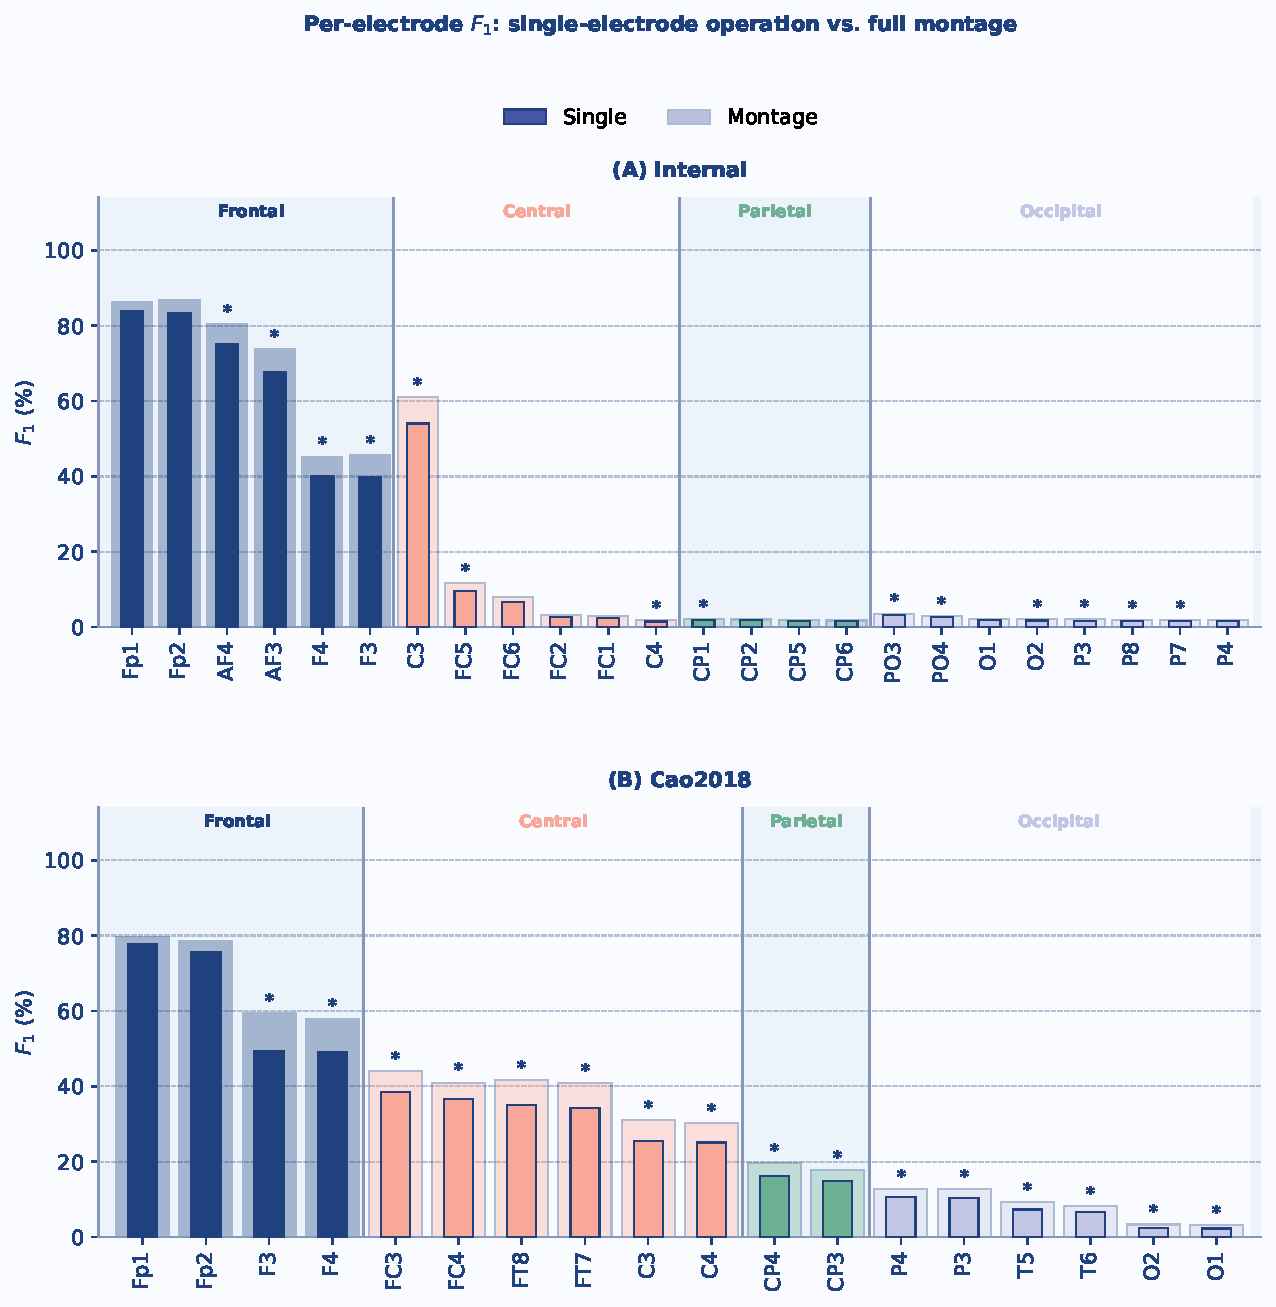
\includegraphics[width=\linewidth]{fig_exp1_single_channel_stats.pdf}
        \caption{Per-electrode comparison of $F_1$ for each electrode in the four curated anatomical regions in the single-electrode run (narrow, opaque bar) and in the full-montage run (wide, translucent bar), for (A)~Internal and (B)~Cao2018.
%
            Comparisons are paired by session using two-tailed Wilcoxon signed-rank tests, with $p$ Bonferroni-corrected separately within each dataset.
%
            An asterisk above an electrode marks adjusted $p<0.05$. Electrodes without an asterisk did not reach this threshold.
%
%
    }
        \label{fig:exp1_single_channel_stats}
    \end{minipage}
    \hfill
    \begin{minipage}[t]{0.48\linewidth}
        \centering
        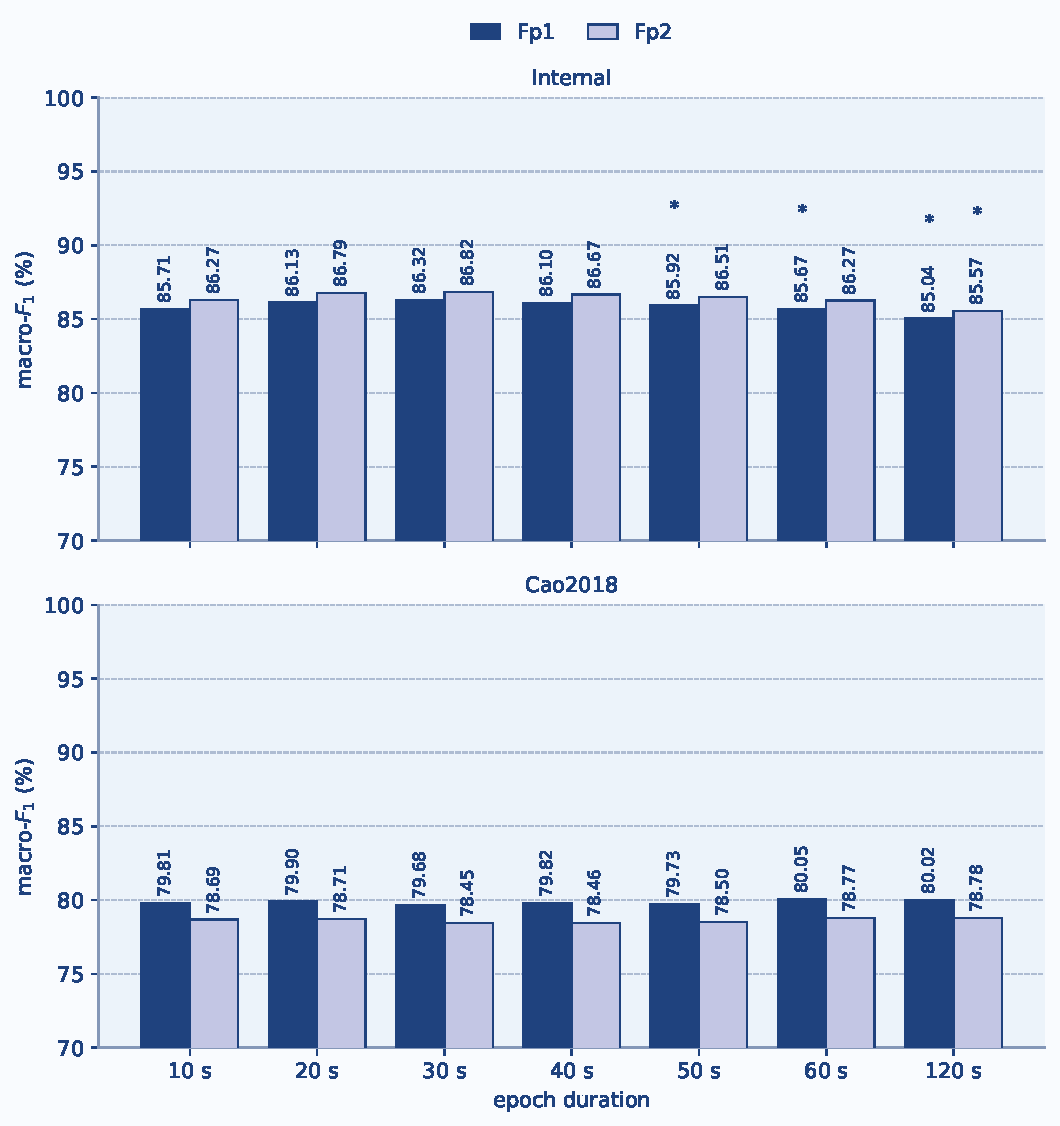
\includegraphics[width=\linewidth]{fig_exp3_epoch_duration.pdf}
        \caption{Macro-averaged $F_1$ of the pipeline across epoch durations, on the full
        32-channel montage, for Fp1 and Fp2 (Experiment~1's two consistently best-performing electrodes) reported separately for Internal (top row) and Cao2018 (bottom row).
        Durations of 10, 20, 30 (reference), 40, 50, 60 and 120 seconds were tested, and an asterisk marks the durations that differ significantly from the
        30\,s reference after Bonferroni correction.}
        \label{fig:f1_by_epoch}
    \end{minipage}
\end{figure*}
%
%
%
%
%
%
%
%
%
%
%
%
%

%
%
%
%
%
%
%
%
%
%
%
%
%
%
%
%
%
%



%
%
%
%
%
%
%


%
%
%

%

%

%

%
%
 

%
%
%
\subsection{Experiment 2: Stability Across Epoch Durations}
\label{sec:exp3_epoch}

%

%
Epoch duration is typically chosen on paradigm-specific or theoretical grounds and is rarely optimised for the blink detector itself. Driving studies use epoch lengths ranging from a few seconds to several minutes~\citep{ahn2016exploring,chai2017improving,lan2024driving,dai2023detection,chen2022fatigue}. Because the physiology of blinks does not depend on the epoch grid imposed during analysis, a robust pipeline should produce stable event-level $F_1$ across this range.




 
%
The pipeline was evaluated under epoch durations of 10, 20, 30, 40, 50, 60, and 120~s, with 30~s serving as the reference duration~\citep{ahn2016exploring,chai2017improving,lan2024driving,dai2023detection,chen2022fatigue}.
%
For each duration, the complete pipeline was rerun from scratch using the full 32-channel montage, since both the Stage~A peak-to-peak statistics and the samples pooled for the Stage~B thresholds change with epoch length. Keeping the full montage ensures that epoch duration is the only factor that differs from the reference. Experiment~1 found that Fp1 and Fp2 were consistently the two best-performing electrodes on both corpora. We therefore restrict the epoch-duration analysis to these two electrodes and report their $F_1$ from each full-montage run. The two electrodes are reported separately rather than averaged.
 
%
Figure~\ref{fig:f1_by_epoch} reports the session-mean $F_1$ of Fp1 and Fp2 for each duration. For each electrode, every non-reference duration was compared with the 30-s reference using a two-tailed Wilcoxon signed-rank test paired by session, with $p$-values Bonferroni-corrected over the six non-reference durations. An asterisk marks durations that differ significantly from the reference (adjusted $p < 0.05$).
 
%
On Internal, the effect of epoch duration depended on the electrode. The 30-s reference yielded the highest $F_1$ for both electrodes, at 86.32\% for Fp1 and 86.82\% for Fp2. Fp1 fell significantly to 85.92\% at 50~s, 85.67\% at 60~s, and 85.04\% at 120~s (adjusted $p < 0.05$ for all three). Fp2 differed significantly only at 120~s, where it fell to 85.57\% (adjusted $p < 0.05$). Its declines at 50 and 60~s, to 86.51\% and 86.27\%, resembled those of Fp1 but did not reach significance after correction (adjusted $p > 0.05$ for both). Neither electrode differed significantly from the reference at 10, 20, or 40~s. Fp2's 60-s decline of 0.55 percentage points was larger than Fp1's significant 50-s decline of 0.40 percentage points, suggesting that significance reflected how consistently the change occurred across sessions rather than its size. Even the significant reductions were small, with the largest being 1.28 percentage points for Fp1 at 120~s.
 
%
On Cao2018, in contrast, neither electrode differed significantly from the 30-s reference at any duration (adjusted $p > 0.05$ for all comparisons). For both electrodes, the reference produced the lowest $F_1$ of the seven durations, at 79.68\% for Fp1 and 78.45\% for Fp2. Shorter epochs gave slightly higher scores, with Fp1 reaching 79.81\% at 10~s and 79.90\% at 20~s, and Fp2 reaching 78.69\% and 78.71\%. Fp1 peaked at 80.05\% at 60~s and Fp2 at 78.78\% at 120~s, only 0.38 and 0.33 percentage points above their reference values. 
%
%
%
%
%
 


%
%
%
%
%
%
%




%
%
%
\subsection{Experiment 3: Strategy Comparison}
\label{sec:exp3_strategy}
%

%
In driving and other epoch-structured paradigms, a common approach is to apply a continuous-signal blink detector to the raw or minimally preprocessed recording and then map the detected blinks back onto the epoch grid. We refer to this as the pooled, continuous-signal strategy, because each channel's detection threshold is estimated once from a signal pool that contains both blink-heavy and blink-free epochs. \rev{The BLINKER-threshold baseline}~\citep{kleifges2017blinker} and the EOG event detector of MNE-Python~\citep{GramfortEtAl2013a} both follow this strategy, although they estimate the threshold in different ways.
\rev{The BLINKER-threshold baseline} combines the mean of the pooled signal with a robust dispersion term, so blink-free epochs dilute these amplitude statistics and pull the threshold down. The MNE detector instead sets its threshold to one quarter of the range of the filtered signal, so a single large excursion anywhere in the recording raises the threshold for every epoch. %
\rev{The hypothesis motivating the proposed pipeline is that either form of pooling may shift the threshold for part of the recording, thereby altering the resulting precision-recall trade-off. The direction and magnitude of this effect depend on the threshold estimator and were not isolated experimentally in this study.}
 
%
We therefore hypothesise that the pooled, continuous-signal strategy produces lower session-level $F_1$ than the epoch-aware pipeline because of a less favourable precision-recall trade-off. To test this hypothesis, \rev{the BLINKER-threshold baseline}, MNE, and the proposed pipeline were applied to every session of Internal and Cao2018 using 30-s epochs. All 32 channels were included to ensure a fair comparison with \rev{the BLINKER-threshold baseline}, which by default processes every channel provided to it. All three methods received the same epochs, band-pass filtered at 1--20~Hz and resampled to 100~Hz, and each baseline was run on the concatenation of these epochs. %
\rev{The BLINKER-threshold baseline was represented by the initial threshold-crossing stage of the BLINKER algorithm; its blink morphological fitting step and automatic channel selection were not used. This baseline therefore evaluates the threshold-estimation component rather than the complete published BLINKER pipeline.} MNE was represented by \texttt{mne.preprocessing.find\_eog\_events}\rev{. Because the function returns point events (peak sample indices), each event was converted to an interval by extending $\pm$100~ms around the detected peak, yielding fixed 200~ms predicted blink windows. The default amplitude threshold of one quarter of the signal range was used.} Both baselines were run on each channel independently.
For each method and session, the channel with the highest $F_1$ was then retained. %
%
 
%
On both datasets, the proposed pipeline achieved the highest session-mean $F_1$, followed by \rev{the BLINKER-threshold baseline} and then MNE. On Internal (Table~\ref{tab:f1_significance}), the proposed pipeline reached 88.25\%, compared with 76.54\% for \rev{the BLINKER-threshold baseline} and 66.64\% for MNE. Its advantage was 11.7 percentage points over \rev{the BLINKER-threshold baseline} and 21.6 percentage points over MNE, and both differences were significant (adjusted $p < 0.05$). On Cao2018 (Table~\ref{tab:f1_significance}), the proposed pipeline likewise reached 80.68\%, against 69.40\% for \rev{the BLINKER-threshold baseline} and 56.27\% for MNE. The margins were 11.3 and 24.4 percentage points, and both were again significant (adjusted $p < 0.05$). All three methods scored lower on Cao2018 than on Internal, but the decline was not uniform. The proposed pipeline and \rev{the BLINKER-threshold baseline} lost 7.6 and 7.1 percentage points, respectively, so the margin between them stayed close to 11 percentage points on both datasets. MNE, in contrast, lost 10.4 percentage points, which widened its gap to the proposed pipeline from 21.6 to 24.4 percentage points and its gap to \rev{the BLINKER-threshold baseline} from 9.9 to 13.1 percentage points.
 
%
The two baselines lost $F_1$ in different ways. On Internal (Figure~\ref{fig:exp3_pr_scatter}), \rev{the BLINKER-threshold baseline} favoured recall over precision, with a mean recall of 95.18\% and a mean precision of 67.94\%. On Cao2018 (Figure~\ref{fig:exp3_pr_scatter}), the same bias was stronger, with a mean recall of 97.15\% against a mean precision of 56.96\%. MNE, in contrast, showed no systematic bias, since its mean recall and precision differed by less than 2 percentage points on both datasets. Its operating points were instead widely dispersed, and recall fell below 30\% in several sessions on each dataset. The proposed pipeline had higher mean precision and recall than MNE on both datasets. Its mean recall was lower than \rev{that of the BLINKER-threshold baseline} (90.14\% on Internal and 89.09\% on Cao2018), but its mean precision was higher (88.03\% and 75.91\%). %
\rev{The recall bias of the BLINKER-threshold baseline is consistent with, but does not prove, the hypothesised pooled-threshold mechanism. A threshold derived from a mixture of blink-heavy and blink-free epochs may differ from an epoch-conditioned estimate, but the specific threshold shift was not measured. The low-recall MNE sessions are consistent with a range-based threshold raised by large excursions elsewhere in the recording, although this mechanism was likewise not isolated.}
%
%
 
%
%
\begin{table}[ht]
  \centering
  \caption{\rev{Session-mean $F_1$ (\%, mean $\pm$ SD) of the proposed pipeline, the BLINKER-threshold baseline, and MNE on Internal ($n=46$ sessions from 17 participants) and Cao2018 ($n=58$ sessions from 27 participants). All conditions are evaluated at the retrospective best-channel-per-session operating point (oracle selection using reference annotations). An asterisk marks a baseline whose session-level $F_1$ differs significantly from that of the proposed pipeline (two-tailed Wilcoxon signed-rank test paired by session, Bonferroni-corrected over the four comparisons shown, adjusted $p < 0.05$).}}
  \label{tab:f1_significance}
  \begin{tabular}{lccc}
    \toprule
    %
    Dataset & Proposed & \rev{BLINKER-threshold} & MNE \\
    \midrule
    %
    \rev{Internal} & \rev{88.25 $\pm$ 10.10} & \rev{76.54 $\pm$ 20.10*} & \rev{66.64 $\pm$ 35.98*} \\
    \rev{Cao2018} & \rev{80.68 $\pm$ 13.04} & \rev{69.40 $\pm$ 19.39*} & \rev{56.27 $\pm$ 32.45*} \\
    \bottomrule
  \end{tabular}
\end{table}
 
\begin{figure}[ht]
  \centering
  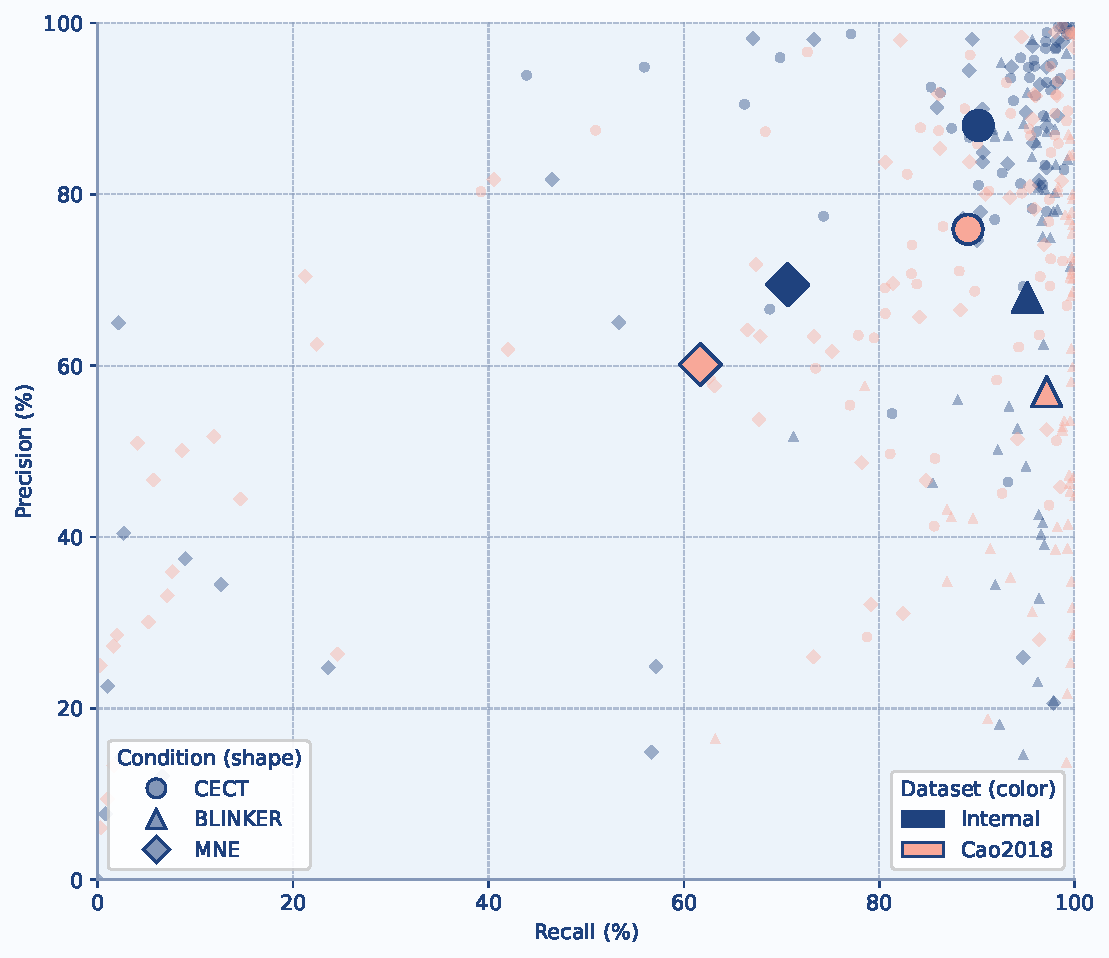
\includegraphics[width=0.9\linewidth]{fig_exp2_pr_scatter.pdf}
  \caption{\rev{Per-session precision-recall operating points of the BLINKER-threshold baseline, MNE, and the proposed pipeline (labelled Proposed-approach in the legend) on Internal and Cao2018. Each small marker is one session's operating point for one method, taken at the retrospective best channel (oracle) in that session. Marker shape encodes the method and marker colour encodes the dataset. The large navy-outlined marker for each method marks its mean over sessions within that dataset.}}
  \label{fig:exp3_pr_scatter}
\end{figure}
 
%
%

%
%
%
%
%
%

 %
\section{Discussion}
\label{sec:discussion}

%
The concentration of blink information at Fp1 and Fp2 agrees with earlier driving studies that detected blinks from a single frontopolar or forehead channel and used them to estimate driver drowsiness or fatigue
~\citep{ko2020eyeblink,shahbakhti2022simultaneous,shahbakhti2023fusion}.
Those studies fixed the frontopolar channel by design. In the present benchmark, the same two electrodes came out on top in every configuration without any such constraint, and neither lost significant performance when the pipeline received only the Frontal region or that electrode alone. Significant losses were common elsewhere under the same reduction, including at the neighbouring frontal electrodes. Because the pipeline derives its candidate epochs and thresholds entirely from the electrodes supplied, the frontopolar advantage does not rely on information borrowed from other channels. The pattern held on both datasets, although the C3--C4 asymmetry was specific to Internal and may reflect a recording or montage characteristic of that dataset. These results also have implications for reduced-channel drowsiness systems, which commonly use occipital electrodes because alpha activity, a well-established marker of driver fatigue~\citep{simon2011eeg}, is prominent over the occipital region~\citep{lin2014wireless,li2015context}. Occipital electrodes performed far below the frontopolar electrodes in every configuration tested here, so a system relying on an occipital channel alone would capture alpha activity but miss most of the blink information available at frontopolar sites. That information is not redundant, since adding blink features to single-channel forehead EEG improved the prediction of driver fatigue in a simulated driving task~\citep{ko2020eyeblink}.
 
%
%
%
%
%
%
%

%

Temporal window duration is an important design consideration in EEG-based driving-state monitoring because it can influence both classification performance and system responsiveness~\citep{rashid2021random}. Previous drowsiness and driving-fatigue studies have compared multiple analysis windows and shown that performance can vary with temporal context~\citep{lee2023lstm,rashid2021random}.
In contrast, EEG eye-blink detectors have generally been evaluated using a single predefined epoch duration rather than systematically across multiple durations ~\citep{chang2016detection,wang2025sliding,shahbakhti2021vme}.
A systematic assessment of how epoch duration affects blink-detection performance, particularly in driving EEG, is therefore still lacking.
In the present study, blink-detection performance at the frontopolar electrodes remained largely stable across 10--40~s epochs.
This differs from drowsiness classification, where performance has been shown to vary more noticeably with analysis-window duration
~\citep{lee2023lstm}. One possible explanation is that blink artifacts typically last only about 100--500~ms~\citep{chang2016detection}, substantially shorter than the epochs evaluated here. Once an epoch is sufficiently long to contain the complete blink waveform, further increases in duration may therefore have limited influence on blink detection itself, although they can alter the amount of background EEG contributing to threshold estimation. From a practical perspective, the observed stability suggests that the proposed pipeline can accommodate a range of epoch durations used in driving-EEG protocols without substantial loss of detection performance.
 
%
%
%
%
%
%
%

%
%
%
%
%
\rev{For fatigue monitoring, the way each baseline failed in the strategy comparison is more informative than the size of the margin.}
The thresholding approach used in \rev{the BLINKER-threshold baseline}~\citep{kleifges2017blinker} retained most blinks but at the expense of lower precision. In a drowsiness-monitoring application, such false detections could artificially inflate blink-rate indices used to assess fatigue~\citep{tian2021fatigue}. \rev{This limitation also helps explain why the complete BLINKER pipeline incorporates additional morphological fitting and channel-selection steps rather than relying on thresholding alone.}
MNE~\citep{GramfortEtAl2013a} instead missed most blinks in several sessions on each dataset. This is arguably the more serious failure for a warning system, which must be reliable for each driver rather than on average~\citep{ingre2006subjective}.
%
\rev{Both failure patterns are consistent with calibrating the threshold on the whole recording, although neither mechanism was isolated experimentally. In the BLINKER-threshold baseline, blink-free epochs may dilute the pool and shift the threshold towards the background EEG, so smaller non-blink deflections could cross it. In MNE, a single large artefact raises the range-based threshold above many genuine blinks. However, the proposed and baseline configurations also differ in several other pipeline components, so the observed precision-recall differences cannot be attributed to the calibration pool alone without a matched ablation~\citep{schleicher2008blinks}.}
%
\rev{The proposed pipeline estimates its threshold only from epochs flagged as containing prominent amplitude excursions, which is intended to reduce the influence of blink-free signal on threshold placement. The proposed configuration outperformed the BLINKER-threshold baseline by a similar $F_1$ margin on Internal and Cao2018, and the ranking was consistent across the two corpora despite differences in hardware and montage.} 
%
These findings are subject to several limitations. The benchmark was restricted to two simulated-driving datasets, so generalisation to other experimental paradigms or clinical populations was not tested. All analyses were also performed offline on recorded data, so performance under real driving conditions, where movement and electrode contact may differ, was not assessed.
Performance was not reported separately by blink duration, so detection of prolonged eye closures, which is particularly relevant to drowsiness assessment, remains unestablished. The evaluation depends on manually annotated reference labels and on their definitions of blink onset and offset, which can vary with signal representation and annotation criteria~\citep{nystrm2024what}. \rev{The Internal labels were anchored to synchronised video and the eye-aspect-ratio signal, whereas the Cao2018 labels relied on EEG morphology alone; this difference in annotation modality limits the comparability of absolute scores across the two corpora.} In addition, the second rater reviewed the first rater's annotations rather than annotating independently from scratch, so inter-rater agreement was not quantified.

%

 
%
There are several related topics that we would like to investigate in future studies, some of which follow directly from the limitations above.
%
The pipeline should first be validated on more independent driving datasets and recording systems, and then on paradigms organised into task blocks or trials, such as the motor-imagery, motor-execution, steady-state visually evoked potential and P300 sessions of a recent multimodal dataset~\citep{guttmann2025dataset}. This would test whether its performance extends to different blink morphologies, cognitive demands, and recording conditions. The pipeline, and reduced-channel systems built on the frontopolar findings, should also be evaluated online under real driving conditions. Online use would require the threshold to be re-estimated over a moving window of recent epochs rather than calibrated on the whole session, and real-time threshold adaptation has already been achieved for unsupervised blink detection~\citep{chang2016unsupervised}. Reporting normal blinks and prolonged closures separately would establish whether performance is retained for the sustained closures most relevant to drowsiness assessment~\citep{tian2021fatigue,shahbakhti2023fusion}.
%
Beyond these limitations, whether a single frontopolar channel can supply the spectral markers of drowsiness as well as blinks should be examined, since it may carry theta and beta activity~\citep{ko2020eyeblink,shahbakhti2022simultaneous,aoki2023drowsiness} but has weaker alpha and strong ocular contamination.
  %


\section{Conclusion}
\label{sec:conclusion}
%
%
%
The spatial analysis further showed that \rev{frontopolar electrodes showed the smallest reduction relative to full-montage performance, although formal equivalence was not tested}, while the epoch-duration analysis indicated broadly stable pooled performance despite some corpus-specific sensitivity to longer epochs. Collectively, these findings support an interpretable and spatially sparse approach to epoch-aware blink detection that can accommodate common segmentation choices without requiring a dense electrode montage.
\rev{The evaluation was restricted to two simulated-driving corpora, and therefore generalisability beyond this domain and suitability for practical deployment remain to be established.}
\rev{Overall, the candidate-epoch-conditioned configuration is a promising and interpretable approach to epoch-aware blink detection in simulated-driving EEG.}
  
%

%
\makeatletter
\def\input@path{{./}}
\makeatother
\bibliographystyle{IEEEtran}
\bibliography{../references_from_csv,../references_scopus_new}

%
%
\clearpage
\makeatletter
\def\input@path{{../}}
\makeatother
\appendices
%
%
%
\section{Per-electrode statistics for the regional and single-electrode analyses}
\label{app:per_electrode_stats}

Tables~\ref{tab:app_regional_internal} and~\ref{tab:app_regional_cao2018} report, for every electrode, the session-level $F_1$ obtained when the pipeline was rerun with only the electrodes of that electrode's region supplied, alongside the $F_1$ of the same electrode in the full-montage run. Tables~\ref{tab:app_single_internal} and~\ref{tab:app_single_cao2018} report the corresponding comparison for the single-electrode runs, in which each electrode was supplied alone.

\begin{table}[htbp]
  \centering
  \renewcommand{\baselinestretch}{1}\normalsize
  \caption{Per-electrode $F_1$ in the regional rerun versus the full-montage run on the Internal dataset. Each electrode's session-level $F_1$ in the regional rerun, in which only the electrodes of that electrode's region were supplied to the pipeline, was paired with its session-level $F_1$ in the full-montage run (all 32 channels supplied) on the sessions common to both runs and compared with a two-tailed Wilcoxon signed-rank test paired by session. An asterisk ($*$) marks electrodes whose difference was significant at the 0.05 level after Bonferroni correction over the 24 electrodes tested within the Internal dataset. $\Delta F_1$ is the reduced-configuration $F_1$ minus the full-montage $F_1$, in percentage points, so negative values indicate lower $F_1$ in the reduced configuration. Within each region, electrodes are ordered by descending regional-rerun $F_1$.}
  \label{tab:app_regional_internal}
  \footnotesize
  \setlength{\tabcolsep}{2.5pt}
  \begin{tabular}{@{}llrrrc@{}}
    \toprule
     &  & $F_1$ regional & $F_1$ full &  & \\
    Region & Electrode & rerun (\%) & montage (\%) & $\Delta F_1$ & Sig. \\
    \midrule
    Frontal & Fp2 & 85.28 & 86.82 & $-1.54$ & \\
     & Fp1 & 84.84 & 86.32 & $-1.48$ & \\
     & AF4 & 77.04 & 80.32 & $-3.28$ & $*$ \\
     & AF3 & 70.70 & 73.76 & $-3.06$ & $*$ \\
     & F3 & 42.68 & 45.65 & $-2.96$ & $*$ \\
     & F4 & 41.00 & 45.23 & $-4.24$ & $*$ \\
    \addlinespace
    Central & C3 & 58.59 & 61.06 & $-2.47$ & $*$ \\
     & FC5 & 10.45 & 11.60 & $-1.14$ & \\
     & FC6 & 7.40 & 8.10 & $-0.71$ & $*$ \\
     & FC1 & 2.89 & 3.07 & $-0.18$ & \\
     & FC2 & 2.89 & 3.11 & $-0.22$ & \\
     & C4 & 1.73 & 1.85 & $-0.12$ & \\
    \addlinespace
    Parietal & CP1 & 1.92 & 2.19 & $-0.27$ & \\
     & CP2 & 1.78 & 2.02 & $-0.24$ & $*$ \\
     & CP5 & 1.64 & 1.80 & $-0.16$ & $*$ \\
     & CP6 & 1.54 & 1.75 & $-0.20$ & $*$ \\
    \addlinespace
    Occipital & PO3 & 3.35 & 3.60 & $-0.25$ & $*$ \\
     & PO4 & 2.81 & 2.98 & $-0.17$ & $*$ \\
     & O2 & 2.05 & 2.13 & $-0.09$ & \\
     & O1 & 2.04 & 2.13 & $-0.09$ & \\
     & P3 & 1.83 & 2.05 & $-0.22$ & \\
     & P8 & 1.82 & 1.94 & $-0.12$ & \\
     & P7 & 1.71 & 1.82 & $-0.11$ & \\
     & P4 & 1.65 & 1.77 & $-0.12$ & \\
    \bottomrule
  \end{tabular}
\end{table}

\begin{table}[htbp]
  \centering
  \renewcommand{\baselinestretch}{1}\normalsize
  \caption{Per-electrode $F_1$ in the regional rerun versus the full-montage run on the Cao2018 dataset. Each electrode's session-level $F_1$ in the regional rerun, in which only the electrodes of that electrode's region were supplied to the pipeline, was paired with its session-level $F_1$ in the full-montage run (all 32 channels supplied) on the sessions common to both runs and compared with a two-tailed Wilcoxon signed-rank test paired by session. An asterisk ($*$) marks electrodes whose difference was significant at the 0.05 level after Bonferroni correction over the 18 electrodes tested within the Cao2018 dataset. $\Delta F_1$ is the reduced-configuration $F_1$ minus the full-montage $F_1$, in percentage points, so negative values indicate lower $F_1$ in the reduced configuration. Within each region, electrodes are ordered by descending regional-rerun $F_1$.}
  \label{tab:app_regional_cao2018}
  \footnotesize
  \setlength{\tabcolsep}{2.5pt}
  \begin{tabular}{@{}llrrrc@{}}
    \toprule
     &  & $F_1$ regional & $F_1$ full &  & \\
    Region & Electrode & rerun (\%) & montage (\%) & $\Delta F_1$ & Sig. \\
    \midrule
    Frontal & Fp1 & 78.80 & 79.68 & $-0.88$ & \\
     & Fp2 & 77.05 & 78.45 & $-1.40$ & \\
     & F3 & 55.97 & 59.51 & $-3.55$ & $*$ \\
     & F4 & 54.64 & 57.99 & $-3.35$ & $*$ \\
    \addlinespace
    Central & FC3 & 40.52 & 44.13 & $-3.61$ & $*$ \\
     & FT8 & 37.44 & 41.63 & $-4.19$ & $*$ \\
     & FC4 & 37.25 & 40.99 & $-3.73$ & $*$ \\
     & FT7 & 36.26 & 40.76 & $-4.49$ & $*$ \\
     & C3 & 27.67 & 31.08 & $-3.42$ & $*$ \\
     & C4 & 26.62 & 30.18 & $-3.56$ & $*$ \\
    \addlinespace
    Parietal & CP4 & 15.63 & 19.56 & $-3.93$ & $*$ \\
     & CP3 & 14.37 & 17.84 & $-3.46$ & $*$ \\
    \addlinespace
    Occipital & P3 & 10.04 & 12.80 & $-2.77$ & $*$ \\
     & P4 & 9.86 & 12.67 & $-2.81$ & $*$ \\
     & T5 & 7.20 & 9.26 & $-2.06$ & $*$ \\
     & T6 & 6.39 & 8.30 & $-1.91$ & $*$ \\
     & O2 & 2.61 & 3.33 & $-0.72$ & $*$ \\
     & O1 & 2.40 & 3.10 & $-0.70$ & $*$ \\
    \bottomrule
  \end{tabular}
\end{table}

\begin{table}[htbp]
  \centering
  \renewcommand{\baselinestretch}{1}\normalsize
  \caption{Per-electrode $F_1$ in the single-electrode run versus the full-montage run on the Internal dataset. Each electrode's session-level $F_1$ in the single-electrode run, in which that electrode alone was supplied to the pipeline, was paired with its session-level $F_1$ in the full-montage run (all 32 channels supplied) on the sessions common to both runs and compared with a two-tailed Wilcoxon signed-rank test paired by session. An asterisk ($*$) marks electrodes whose difference was significant at the 0.05 level after Bonferroni correction over the 24 electrodes tested within the Internal dataset. $\Delta F_1$ is the reduced-configuration $F_1$ minus the full-montage $F_1$, in percentage points, so negative values indicate lower $F_1$ in the reduced configuration. Within each region, electrodes are ordered by descending single-electrode-run $F_1$.}
  \label{tab:app_single_internal}
  \footnotesize
  \setlength{\tabcolsep}{2.5pt}
  \begin{tabular}{@{}llrrrc@{}}
    \toprule
     &  & $F_1$ single- & $F_1$ full &  & \\
    Region & Electrode & electrode (\%) & montage (\%) & $\Delta F_1$ & Sig. \\
    \midrule
    Frontal & Fp1 & 83.73 & 86.32 & $-2.59$ & \\
     & Fp2 & 83.37 & 86.82 & $-3.45$ & \\
     & AF4 & 75.16 & 80.32 & $-5.16$ & $*$ \\
     & AF3 & 67.59 & 73.76 & $-6.17$ & $*$ \\
     & F4 & 39.98 & 45.23 & $-5.26$ & $*$ \\
     & F3 & 39.85 & 45.65 & $-5.79$ & $*$ \\
    \addlinespace
    Central & C3 & 54.05 & 61.06 & $-7.02$ & $*$ \\
     & FC5 & 9.51 & 11.60 & $-2.09$ & $*$ \\
     & FC6 & 6.73 & 8.10 & $-1.37$ & \\
     & FC2 & 2.69 & 3.11 & $-0.42$ & \\
     & FC1 & 2.42 & 3.07 & $-0.65$ & \\
     & C4 & 1.51 & 1.85 & $-0.34$ & $*$ \\
    \addlinespace
    Parietal & CP1 & 1.86 & 2.19 & $-0.32$ & $*$ \\
     & CP2 & 1.86 & 2.02 & $-0.15$ & \\
     & CP5 & 1.57 & 1.80 & $-0.23$ & \\
     & CP6 & 1.53 & 1.75 & $-0.22$ & \\
    \addlinespace
    Occipital & PO3 & 3.15 & 3.60 & $-0.45$ & $*$ \\
     & PO4 & 2.65 & 2.98 & $-0.34$ & $*$ \\
     & O1 & 1.97 & 2.13 & $-0.16$ & \\
     & O2 & 1.78 & 2.13 & $-0.36$ & $*$ \\
     & P3 & 1.66 & 2.05 & $-0.39$ & $*$ \\
     & P8 & 1.62 & 1.94 & $-0.32$ & $*$ \\
     & P7 & 1.61 & 1.82 & $-0.21$ & $*$ \\
     & P4 & 1.57 & 1.77 & $-0.20$ & \\
    \bottomrule
  \end{tabular}
\end{table}

\begin{table}[htbp]
  \centering
  \renewcommand{\baselinestretch}{1}\normalsize
  \caption{Per-electrode $F_1$ in the single-electrode run versus the full-montage run on the Cao2018 dataset. Each electrode's session-level $F_1$ in the single-electrode run, in which that electrode alone was supplied to the pipeline, was paired with its session-level $F_1$ in the full-montage run (all 32 channels supplied) on the sessions common to both runs and compared with a two-tailed Wilcoxon signed-rank test paired by session. An asterisk ($*$) marks electrodes whose difference was significant at the 0.05 level after Bonferroni correction over the 18 electrodes tested within the Cao2018 dataset. $\Delta F_1$ is the reduced-configuration $F_1$ minus the full-montage $F_1$, in percentage points, so negative values indicate lower $F_1$ in the reduced configuration. Within each region, electrodes are ordered by descending single-electrode-run $F_1$.}
  \label{tab:app_single_cao2018}
  \footnotesize
  \setlength{\tabcolsep}{2.5pt}
  \begin{tabular}{@{}llrrrc@{}}
    \toprule
     &  & $F_1$ single- & $F_1$ full &  & \\
    Region & Electrode & electrode (\%) & montage (\%) & $\Delta F_1$ & Sig. \\
    \midrule
    Frontal & Fp1 & 77.65 & 79.68 & $-2.03$ & \\
     & Fp2 & 75.59 & 78.45 & $-2.86$ & \\
     & F3 & 49.30 & 59.51 & $-10.21$ & $*$ \\
     & F4 & 49.03 & 57.99 & $-8.96$ & $*$ \\
    \addlinespace
    Central & FC3 & 38.44 & 44.13 & $-5.70$ & $*$ \\
     & FC4 & 36.72 & 40.99 & $-4.27$ & $*$ \\
     & FT8 & 34.99 & 41.63 & $-6.63$ & $*$ \\
     & FT7 & 34.22 & 40.76 & $-6.54$ & $*$ \\
     & C3 & 25.43 & 31.08 & $-5.66$ & $*$ \\
     & C4 & 25.10 & 30.18 & $-5.08$ & $*$ \\
    \addlinespace
    Parietal & CP4 & 16.22 & 19.56 & $-3.34$ & $*$ \\
     & CP3 & 14.80 & 17.84 & $-3.04$ & $*$ \\
    \addlinespace
    Occipital & P4 & 10.66 & 12.67 & $-2.01$ & $*$ \\
     & P3 & 10.28 & 12.80 & $-2.52$ & $*$ \\
     & T5 & 7.32 & 9.26 & $-1.94$ & $*$ \\
     & T6 & 6.66 & 8.30 & $-1.64$ & $*$ \\
     & O2 & 2.42 & 3.33 & $-0.91$ & $*$ \\
     & O1 & 2.28 & 3.10 & $-0.82$ & $*$ \\
    \bottomrule
  \end{tabular}
\end{table}
 
%
%
\makeatletter
\def\input@path{{./}}
\makeatother

\end{document}
